%!TEX root = ../dokumentation.tex

%
% Nahezu alle Einstellungen koennen hier getaetigt werden
%

\RequirePackage[l2tabu, orthodox]{nag}	% weist in Commandozeile bzw. log auf veraltete LaTeX Syntax hin

\documentclass[%
	pdftex,
	oneside,			% Einseitiger Druck.
	12pt,				% Schriftgroesse
	parskip=half,		% Halbe Zeile Abstand zwischen Absätzen.
%	topmargin = 10pt,	% Abstand Seitenrand (Std:1in) zu Kopfzeile [laut log: unused]
	headheight = 12pt,	% Höhe der Kopfzeile
%	headsep = 30pt,	% Abstand zwischen Kopfzeile und Text Body  [laut log: unused]
	headsepline,		% Linie nach Kopfzeile.
	footsepline,		% Linie vor Fusszeile.
	footheight = 16pt,	% Höhe der Fusszeile
	abstracton,		% Abstract Überschriften
	DIV=calc,		% Satzspiegel berechnen
	BCOR=8mm,		% Bindekorrektur links: 8mm
	headinclude=false,	% Kopfzeile nicht in den Satzspiegel einbeziehen
	footinclude=false,	% Fußzeile nicht in den Satzspiegel einbeziehen
	listof=totoc,		% Abbildungs-/ Tabellenverzeichnis im Inhaltsverzeichnis darstellen
	toc=bibliography,	% Literaturverzeichnis im Inhaltsverzeichnis darstellen
]{scrreprt}	% Koma-Script report-Klasse, fuer laengere Bachelorarbeiten alternativ auch: scrbook

% Einstellungen laden
\usepackage{xstring}
\usepackage[utf8]{inputenc}
\usepackage[T1]{fontenc}

\newcommand{\einstellung}[1]{%
  \expandafter\newcommand\csname #1\endcsname{}
  \expandafter\newcommand\csname setze#1\endcsname[1]{\expandafter\renewcommand\csname#1\endcsname{##1}}
}
\newcommand{\langstr}[1]{\einstellung{lang#1}}

\einstellung{martrikelnr}
\einstellung{titel}
\einstellung{kurs}
\einstellung{datumAbgabe}
\einstellung{firma}
\einstellung{firmenort}
\einstellung{abgabeort}
\einstellung{abschluss}
\einstellung{studiengang}
\einstellung{dhbw}
\einstellung{betreuer}
\einstellung{gutachter}
\einstellung{zeitraum}
\einstellung{arbeit}
\einstellung{autor}
\einstellung{sprache}
\einstellung{schriftart}
\einstellung{seitenrand}
\einstellung{kapitelabstand}
\einstellung{spaltenabstand}
\einstellung{zeilenabstand}
\einstellung{zitierstil}
 % verfügbare Einstellungen
%%%%%%%%%%%%%%%%%%%%%%%%%%%%%%%%%%%%%%%%%%%%%%%%%%%%%%%%%%%%%%%%%%%%%%%%%%%%%%%
%                                   Einstellungen
%
% Hier können alle relevanten Einstellungen für diese Arbeit gesetzt werden.
% Dazu gehören Angaben u.a. über den Autor sowie Formatierungen.
%
%
%%%%%%%%%%%%%%%%%%%%%%%%%%%%%%%%%%%%%%%%%%%%%%%%%%%%%%%%%%%%%%%%%%%%%%%%%%%%%%%


%%%%%%%%%%%%%%%%%%%%%%%%%%%%%%%%%%%% Sprache %%%%%%%%%%%%%%%%%%%%%%%%%%%%%%%%%%%
%% Aktuell sind Deutsch und Englisch unterstützt.
%% Es werden nicht nur alle vom Dokument erzeugten Texte in
%% der entsprechenden Sprache angezeigt, sondern auch weitere
%% Aspekte angepasst, wie z.B. die Anführungszeichen und
%% Datumsformate.
\setzesprache{en} % oder en
%%%%%%%%%%%%%%%%%%%%%%%%%%%%%%%%%%%%%%%%%%%%%%%%%%%%%%%%%%%%%%%%%%%%%%%%%%%%%%%%

%%%%%%%%%%%%%%%%%%%%%%%%%%%%%%%%%%% Angaben  %%%%%%%%%%%%%%%%%%%%%%%%%%%%%%%%%%%
%% Die meisten der folgenden Daten werden auf dem
%% Deckblatt angezeigt, einige auch im weiteren Verlauf
%% des Dokuments.
\setzetitel{Database Implementation}
%\setzetitel{Logfileanalyse mit Apache{\textsuperscript{TM}} Hadoop\textsuperscript{{\textregistered}} MapReduce}
\setzedatumAbgabe{11. April 2017}
\setzeabgabeort{Stuttgart}
%\setzeabschluss{Abschluss}
\setzestudiengang{Applied Computer Science}
\setzedhbw{Stuttgart}
\setzegutachter{Dr. Carmen Winter}
%\setzezeitraum{2 Wochen}
\setzearbeit{The NoSQL-Database E-Book}
\setzeautor{IT14C}
%%%%%%%%%%%%%%%%%%%%%%%%%%%%%%%%%%%%%%%%%%%%%%%%%%%%%%%%%%%%%%%%%%%%%%%%%%%%%%%%

%%%%%%%%%%%%%%%%%%%%%%%%%%%% Literaturverzeichnis %%%%%%%%%%%%%%%%%%%%%%%%%%%%%%
%% Bei Fehlern während der Verarbeitung bitte in ads/header.tex bei der
%% Einbindung des Pakets biblatex (ungefähr ab Zeile 110,
%% einmal für jede Sprache), biber in bibtex ändern.
\newcommand{\ladeliteratur}{%
\addbibresource{bibliographie.bib}
%\addbibresource{weitereDatei.bib}
}
%% Zitierstil
%% siehe: http://ctan.mirrorcatalogs.com/macros/latex/contrib/biblatex/doc/biblatex.pdf (3.3.1 Citation Styles)
%% mögliche Werte z.B numeric-comp, alphabetic, authoryear
\setzezitierstil{authoryear}
%%%%%%%%%%%%%%%%%%%%%%%%%%%%%%%%%%%%%%%%%%%%%%%%%%%%%%%%%%%%%%%%%%%%%%%%%%%%%%%%

%%%%%%%%%%%%%%%%%%%%%%%%%%%%%%%%% Layout %%%%%%%%%%%%%%%%%%%%%%%%%%%%%%%%%%%%%%%
%% Verschiedene Schriftarten
% laut nag Warnung: palatino obsolete, use mathpazo, helvet (option scaled=.95), courier instead
\setzeschriftart{lmodern} % palatino oder goudysans, lmodern, libertine

%% Paket um Textteile drehen zu können
%\usepackage{rotating}
%% Paket um Seite im Querformat anzuzeigen
%\usepackage{lscape}

%% Seitenränder
\setzeseitenrand{2.5cm}

%% Abstand vor Kapitelüberschriften zum oberen Seitenrand
\setzekapitelabstand{20pt}

%% Spaltenabstand
\setzespaltenabstand{10pt}
%%Zeilenabstand innerhalb einer Tabelle
\setzezeilenabstand{1.5}
%%%%%%%%%%%%%%%%%%%%%%%%%%%%%%%%%%%%%%%%%%%%%%%%%%%%%%%%%%%%%%%%%%%%%%%%%%%%%%%%

%%%%%%%%%%%%%%%%%%%%%%%%%%%%% Verschiedenes  %%%%%%%%%%%%%%%%%%%%%%%%%%%%%%%%%%%
%% Farben (Angabe in HTML-Notation mit großen Buchstaben)
\newcommand{\ladefarben}{%
	\definecolor{LinkColor}{HTML}{00007A}
	\definecolor{ListingBackground}{HTML}{FCFAFB}
}
%% Mathematikpakete benutzen (Pakete aktivieren)
\usepackage{amsmath}
\usepackage{amssymb}

%% Programmiersprachen Highlighting (Listings)
\newcommand{\listingsettings}{%
	\lstset{%
		language=C,			% Standardsprache des Quellcodes
		numbers=left,			% Zeilennummern links
		stepnumber=1,			% Jede Zeile nummerieren.
		numbersep=5pt,			% 5pt Abstand zum Quellcode
		numberstyle=\tiny,		% Zeichengrösse 'tiny' für die Nummern.
		breaklines=true,		% Zeilen umbrechen wenn notwendig.
		breakautoindent=true,	% Nach dem Zeilenumbruch Zeile einrücken.
		postbreak=\space,		% Bei Leerzeichen umbrechen.
		tabsize=2,				% Tabulatorgrösse 2
		basicstyle=\ttfamily\footnotesize, % Nichtproportionale Schrift, klein für den Quellcode
		showspaces=false,		% Leerzeichen nicht anzeigen.
		showstringspaces=false,	% Leerzeichen auch in Strings ('') nicht anzeigen.
		extendedchars=true,		% Alle Zeichen vom Latin1 Zeichensatz anzeigen.
		captionpos=b,			% sets the caption-position to bottom
		backgroundcolor=\color{ListingBackground}, % Hintergrundfarbe des Quellcodes setzen.
		xleftmargin=0pt,		% Rand links
		xrightmargin=0pt,		% Rand rechts
		frame=single,			% Rahmen an
		frameround=ffff,
		rulecolor=\color{darkgray},	% Rahmenfarbe
		fillcolor=\color{ListingBackground},
		keywordstyle=\color[rgb]{0.133,0.133,0.6}\bfseries,
		commentstyle=\color{Sepia},
		stringstyle=\color{red}
	}
}
%%%%%%%%%%%%%%%%%%%%%%%%%%%%%%%%%%%%%%%%%%%%%%%%%%%%%%%%%%%%%%%%%%%%%%%%%%%%%%%%

%%%%%%%%%%%%%%%%%%%%%%%%%%%%%%%% Eigenes %%%%%%%%%%%%%%%%%%%%%%%%%%%%%%%%%%%%%%%
%% Hier können Ergänzungen zur Präambel vorgenommen werden (eigene Pakete, Einstellungen)

% xcolor muss mit optionen vor pdfpages geladen werden
\usepackage[usenames,dvipsnames,table,xcdraw]{xcolor} 	%xcolor für HTML-Notation

\usepackage{pdfpages}
 % lese Einstellungen

\newcommand{\iflang}[2]{%
  \IfStrEq{\sprache}{#1}{#2}{}
}

\langstr{abkverz}
\langstr{anhang}
\langstr{glossar}
\langstr{deckblattabschlusshinleitung}
\langstr{artikelstudiengang}
\langstr{studiengang}
\langstr{anderdh}
\langstr{von}
\langstr{dbbearbeitungszeit}
\langstr{dbmatriknr}
\langstr{dbkurs}
\langstr{dbfirma}
\langstr{dbbetreuer}
\langstr{dbgutachter}
\langstr{sperrvermerk}
\langstr{erklaerung}
\langstr{abstract}
\langstr{listingname}
\langstr{listlistingname}
\langstr{listingautorefname}
 % verfügbare Strings
\input{lang/\sprache} % Übersetzung einlesen

% Einstellung der Sprache des Paketes Babel und der Verzeichnisüberschriften
\iflang{de}{\usepackage[english, ngerman]{babel}}
\iflang{en}{\usepackage[ngerman, english]{babel}} 


%%%%%%% Package Includes %%%%%%%

\usepackage[margin=\seitenrand,foot=1cm]{geometry}	% Seitenränder und Abstände
\usepackage[activate]{microtype} %Zeilenumbruch und mehr
\usepackage[onehalfspacing]{setspace}
\usepackage{makeidx}
\usepackage[autostyle=true,german=quotes]{csquotes}
\usepackage{tabularx}
\usepackage{longtable}
\usepackage{multirow}
\usepackage{enumitem}	% mehr Optionen bei Aufzählungen
\usepackage{graphicx}
%\usepackage[usenames,dvipsnames,table,xcdraw]{xcolor} 	%xcolor für HTML-Notation
\usepackage{float}
\usepackage{array}
\usepackage{calc}		% zum Rechnen (Bildtabelle in Deckblatt)
\usepackage[right]{eurosym}
\usepackage{wrapfig}
\usepackage{pgffor} % für automatische Kapiteldateieinbindung
\usepackage[perpage, hang, multiple, stable]{footmisc} % Fussnoten
%\usepackage[nohyperlinks]{acronym} % falls gewünscht kann die Option footnote eingefügt werden, dann wird die Erklärung nicht inline sondern in einer Fußnote dargestellt
\usepackage{acronym}

\usepackage{listings}

% Eigene zusätzliche packages
\usepackage{xfrac}
\usepackage{tikz}
\usepackage{subcaption}
%\usepackage[leqno]{amsmath}
%\usepackage{remreset}

% Wurzel mit schießendem Strich am ende
% New definition of square root: % it renames \sqrt as \oldsqrt
\let\oldsqrt\sqrt % it defines the new \sqrt in terms of the old one 
\def\sqrt{\mathpalette\DHLhksqrt} \def\DHLhksqrt#1#2{
\setbox0=\hbox{$#1\oldsqrt{#2\,}$}\dimen0=\ht0 \advance\dimen0-0.2\ht0 \setbox2=\hbox{\vrule height\ht0 depth -\dimen0}{\box0\lower0.4pt\box2}}

%\makeatletter
%\@removefromreset{equation}{chapter}
%\makeatother
%\renewcommand*{\theequation}{\arabic{equation}}

% eine Kommentarumgebung "k" (Handhabe mit \begin{k}<Kommentartext>\end{k},
% Kommentare werden rot gedruckt). Wird \% vor excludecomment{k} entfernt,
% werden keine Kommentare mehr gedruckt.
\usepackage{comment}
\specialcomment{k}{\begingroup\color{red}}{\endgroup}
%\excludecomment{k}


%%%%%% Configuration %%%%%

%% Anwenden der Einstellungen

\usepackage{\schriftart}
\ladefarben{}

% Titel, Autor und Datum
\title{\titel}
\author{\autor}
\date{\datum}

% PDF Einstellungen
\usepackage[%
	pdftitle={\titel},
	pdfauthor={\autor},
	pdfsubject={\arbeit},
	pdfcreator={pdflatex, LaTeX with KOMA-Script},
	pdfpagemode=UseOutlines, 		% Beim Oeffnen Inhaltsverzeichnis anzeigen
	pdfdisplaydoctitle=true, 		% Dokumenttitel statt Dateiname anzeigen.
	pdflang={\sprache}, 			% Sprache des Dokuments.
]{hyperref}

% (Farb-)einstellungen für die Links im PDF
\hypersetup{%
	colorlinks=true, 		% Aktivieren von farbigen Links im Dokument
	linkcolor=LinkColor, 	% Farbe festlegen
	citecolor=LinkColor,
	filecolor=LinkColor,
	menucolor=LinkColor,
	urlcolor=LinkColor,
	linktocpage=true, 		% Nicht der Text sondern die Seitenzahlen in Verzeichnissen klickbar
	bookmarksnumbered=true 	% Überschriftsnummerierung im PDF Inhalt anzeigen.
}
% Workaround um Fehler in Hyperref, muss hier stehen bleiben
\usepackage{bookmark} %nur ein latex-Durchlauf für die Aktualisierung von Verzeichnissen nötig

% Schriftart in Captions etwas kleiner
\addtokomafont{caption}{\small}

% % Literaturverweise (sowohl deutsch als auch englisch)
% \iflang{de}{%
% \usepackage[
% 	backend=bibtex,		% empfohlen. Falls biber Probleme macht: bibtex
% 	bibwarn=true,
% 	bibencoding=utf8,	% wenn .bib in utf8, sonst ascii
% 	sortlocale=de_DE,
% 	style=\zitierstil,
% 	backref=true
% ]{biblatex}
% }
% \iflang{en}{%
% \usepackage[
% 	backend=bibtex,		% empfohlen. Falls biber Probleme macht: bibtex
% 	bibwarn=true,
% 	bibencoding=utf8,	% wenn .bib in utf8, sonst ascii
% 	sortlocale=en_US,
% 	style=\zitierstil,
% ]{biblatex}
% }

% % Mehr Platz zwischen einzelnen Items im Literaturverzeichnis bei Verwendung von authoryear
% \setlength{\bibitemsep}{\baselineskip}
% \DeclareNameAlias{sortname}{last-first}
% 
% \ladeliteratur{}
\usepackage{apacite}
% Glossar
\usepackage[nonumberlist,toc]{glossaries}

%%%%%% Additional settings %%%%%%

% Hurenkinder und Schusterjungen verhindern
% http://projekte.dante.de/DanteFAQ/Silbentrennung
\clubpenalty = 10000 % schließt Schusterjungen aus (Seitenumbruch nach der ersten Zeile eines neuen Absatzes)
\widowpenalty = 10000 % schließt Hurenkinder aus (die letzte Zeile eines Absatzes steht auf einer neuen Seite)
\displaywidowpenalty=10000

% Bildpfad
\graphicspath{{images/}}

% Einige häufig verwendete Sprachen
\lstloadlanguages{PHP,Python,Java,C,C++,bash,XML}
\listingsettings{}
% Umbennung des Listings
\renewcommand\lstlistingname{\langlistingname}
\renewcommand\lstlistlistingname{\langlistlistingname}
\def\lstlistingautorefname{\langlistingautorefname}

% Umlaute ermöglichen in listings
\lstset{literate=
	{á}{{\'a}}1 {é}{{\'e}}1 {í}{{\'i}}1 {ó}{{\'o}}1 {ú}{{\'u}}1
	{Á}{{\'A}}1 {É}{{\'E}}1 {Í}{{\'I}}1 {Ó}{{\'O}}1 {Ú}{{\'U}}1
	{à}{{\`a}}1 {è}{{\`e}}1 {ì}{{\`i}}1 {ò}{{\`o}}1 {ù}{{\`u}}1
	{À}{{\`A}}1 {È}{{\'E}}1 {Ì}{{\`I}}1 {Ò}{{\`O}}1 {Ù}{{\`U}}1
	{ä}{{\"a}}1 {ë}{{\"e}}1 {ï}{{\"i}}1 {ö}{{\"o}}1 {ü}{{\"u}}1
	{Ä}{{\"A}}1 {Ë}{{\"E}}1 {Ï}{{\"I}}1 {Ö}{{\"O}}1 {Ü}{{\"U}}1
	{â}{{\^a}}1 {ê}{{\^e}}1 {î}{{\^i}}1 {ô}{{\^o}}1 {û}{{\^u}}1
	{Â}{{\^A}}1 {Ê}{{\^E}}1 {Î}{{\^I}}1 {Ô}{{\^O}}1 {Û}{{\^U}}1
	{œ}{{\oe}}1 {Œ}{{\OE}}1 {æ}{{\ae}}1 {Æ}{{\AE}}1 {ß}{{\ss}}1
	{ç}{{\c c}}1 {Ç}{{\c C}}1 {ø}{{\o}}1 {å}{{\r a}}1 {Å}{{\r A}}1
	{€}{{\EUR}}1 {£}{{\pounds}}1
}

% Weitere Keyword Highlights
\lstset{
	emph=[1]{ 
	    mkdir, jps, sudo, wget, mv, chown, su, adduser, addgroup, grep, sort, print, max, WARNING
    },
    emphstyle=[1]{\color[rgb]{0.133,0.133,0.6}},
    emph=[2]{
	    LFAConfiguration, Driver, Set, Exception, Configuration, FileInputFormat, FileOutputFormat, Job, Path, Text, IntWritable, Mapper, Matcher, Pattern, PatternMapper, Logger, Level, Context, IOException, InterruptedException, Reducer, CountReducer, TextInputFormat, TextOutputFormat, RecordReader, PDFInputFormat, PDFLineRecordReader, InputSplit, TaskAttemptContext, JobContext, CharSequence
    },
    emphstyle=[2]{\color[HTML]{006400}},
    emph=[3]{
	    String, int, Object, Iterable, boolean, Class, float
    },
    emphstyle=[3]{\color{Mulberry}}
}

% Abstände in Tabellen
\setlength{\tabcolsep}{\spaltenabstand}
\renewcommand{\arraystretch}{\zeilenabstand}


\makeglossaries
%!TEX root = ../dokumentation.tex

%
% vorher in Konsole folgendes aufrufen:
%	makeglossaries makeglossaries dokumentation.acn && makeglossaries dokumentation.glo
%

%
% Glossareintraege --> referenz, name, beschreibung
% Aufruf mit \gls{...}
%
\newglossaryentry{Glossareintrag}{name={Glossareintrag},plural={Glossareinträge},description={Ein Glossar beschreibt verschiedenste Dinge in kurzen Worten}}

\newglossaryentry{Commodity-Hardware}{name={Commodity-Hardware},description={\flqq Computer hardware that is affordable and easy to obtain. Typically it is a low-performance system that is IBM PC-compatible and is capable of running Microsoft Windows, Linux, or MS-DOS without requiring any special devices or equipment.\frqq\footcite{Beal.2015}}}

\newglossaryentry{Git}{name={Git},plural={Git},description={Git ist ein kostenloses System zur Versionskontrolle für kleine wie auch sehr große Projekte. ({\url{http://git-scm.com/}})}}

\newglossaryentry{NetBeans}{name={NetBeans},plural={NetBeans},description={The Smarter and Faster Way to Code Quickly and easily develop desktop, mobile and web applications with Java, HTML5, PHP, C/C++ and more. NetBeans IDE is FREE, open source, and has a worldwide community of users and developers. ({\url{https://netbeans.org}})}}

\newglossaryentry{Maven}{name={Maven},plural={Maven},description={Apache Maven is a software project management and comprehension tool. Based on the concept of a project object model (POM), Maven can manage a project’s build, reporting and documentation from a central piece of information. \\ ({\url{http://maven.apache.org/}})}}

\newglossaryentry{Nagios}{name={Nagios},plural={Nagios},description={Nagios Is The Industry Standard In IT Infrastructure Monitoring. Achieve instant awareness of IT infrastructure problems, so downtime doesn't adversely affect your business. Nagios offers complete monitoring and alerting for servers, switches, applications, and services. \\ ({\url{https://www.nagios.org}})}}

\newglossaryentry{Zabbix}{name={Zabbix},plural={Zabbix},description={Zabbix is the ultimate enterprise-level software designed for real-time monitoring of millions of metrics collected from tens of thousands of servers, virtual machines and network devices. Zabbix is Open Source and comes at no cost. \\ ({\url{http://www.zabbix.com}})}}

\newglossaryentry{Bootstrapping}{name={Bootstrapping},description={\flqq The computer term bootstrap began as a metaphor in the 1950s. In computers, pressing a bootstrap button caused a hardwired program to read a bootstrap program from an input unit. The computer would then execute the bootstrap program, which caused it to read more program instructions. It became a self-sustaining process that proceeded without external help from manually entered instructions. As a computing term, bootstrap has been used since at least 1953.\frqq\footcite[S. 1273]{Buchholz.1953}}}

\newglossaryentry{Generic}{name={Generic},plural={Generics},description={Ein Interface oder eine Klasse kann mit einem oder mehreren Parametern, den sog. Generics, definiert werden, welche zusätzliche Typangaben enthalten. Diese werden in spitzen Klammern notiert. Generics führen implizit einen Typumwandlung durch, welcher ohne Generics explizit erfolgen müsste\footcite[Vgl.][S. 4 f.]{Naftalin.2006}}}

\newglossaryentry{Plugin}{name={Plugin},plural={Plugins},description={\flqq Zusatzprogramm, welches über eine vordefinierte Schnittstelle in ein Basisprogramm eingebunden wird und dessen Funktionsumfang erweitert. [...] [Stammen] oftmals von anderen Herstellern als das Basisprogramm. [...] Plug-ins sind oft aus eigenständigen Programmen entstanden und können deshalb [...] i.d.R. auch ohne das Basisprogramm verwendet werden\frqq\footcite[]{Lackes.2015}}}

\usepackage[table,xcdraw]{xcolor}
\usepackage{tikz}
\usepackage{url}
\usepackage{mdframed}

%CODEDESIGN:
%\definecolor{codeBackground}{rgb}{0.9, 0.9, 0.8}
%\lstnewenvironment{mylisting}[1]{
%	\lstset{
%		basicstyle=\ttfamily\small,
%		breaklines=true,
%		moredelim=**[is][\bfseries]{|}{|},% bold everything in between ||
%		moredelim=**[is][\itshape]{*}{*}  % italic everything in between **
%	}%
%	\mdframed[backgroundcolor=codeBackground,shadow=true,shadowsize=2pt,shadowcolor=black!30]%
%}{%
%\bigskip
%\ignorespaces
%}

%%%%

% custom commands

\definecolor{codegray}{gray}{0.9}
\newcommand{\code}[1]{\colorbox{codegray}{\texttt{#1}}}

\begin{document}

	% Deckblatt
	\begin{spacing}{1}
		%!TEX root = ../dokumentation.tex

\begin{titlepage}
	\begin{longtable}{p{8.2cm} p{5.4cm}}
%		{\raisebox{\ht\strutbox-\totalheight}{
\includegraphics[scale=3]{images/firma-deckblatt.jpg}}} &
		{\raisebox{\ht\strutbox-\totalheight}{
\includegraphics[height=2.5cm]{images/dhbw.png}}}
	\end{longtable}
	\enlargethispage{20mm}
	\begin{center}
		\vspace*{12mm}	{\LARGE\textbf \titel }\\
		\vspace*{12mm}
		\vspace*{12mm}	{\large\textbf \arbeit}\\
		%\vspace*{12mm}	\langdeckblattabschlusshinleitung\\
		\vspace*{12mm}
		%\vspace*{3mm}		{\textbf \abschluss}\\
		%\vspace*{12mm}	\langartikelstudiengang{} \langstudiengang{} \studiengang\\
    \vspace*{3mm}		\langanderdh{} \dhbw\\
		\vspace*{12mm}	\langvon\\
		\vspace*{3mm}		{\textbf \autor}\\
		\vspace*{12mm}	\datumAbgabe\\
	\end{center}
	\vfill
\end{titlepage}

	\end{spacing}
	\newpage
		\section*{Thanks to all contributers}

\begin{center}
	\begin{itemize}
		\item[] AH
		\item[] AS
		\item[] CB
		\item[] CW
		\item[] DH
		\item[] FR
		\item[] FS
		\item[] FS
		\item[] IF
		\item[] JH
		\item[] JJ
		\item[] KO
		\item[] LE
		\item[] LG 
		\item[] MH
		\item[] MJ
		\item[] ML
		\item[] MK
		\item[] MV
		\item[] MW
		\item[] SO
		\item[] SR
		\item[] ST
		\item[] TF
		\item[] TW
	\end{itemize}
\end{center}
	\newpage
	\pagestyle{plain}	

	% Inhaltsverzeichnis
	\begin{spacing}{1.1}
		\begingroup
			\setcounter{tocdepth}{2}
			\tableofcontents
			\clearpage
		\endgroup
	\end{spacing}
	\newpage

	\pagenumbering{arabic}
	
	\pagestyle{headings}

	% Struktur
	\part{Column Oriented DB}
\chapter{HBase}
%!TEX root = ../dokumentation.tex

\chapter{Introduction}
\section{Column-oriented DBMS}

Column oriented databases store data of a table in columns, instead of storing them in rows. 
This describes the fact how data is saved on the hard disk.

In normal row-oriented DBMS the data is grouped into a bunch of data. 
Each of that bunch is saved in a separate file, more concrete it contains a few rows with all columns of this table. 
\cite{hbase.stavros.harizopoulos.2009}

This means that a read access needs to read a lot of unwanted data.
For example, if it is necessary to access just first names, all data of every row must be read and then discarded, until the name is found. 
Aferwards it is necessary to read another first name and so on. 
\cite{hbase.stavros.harizopoulos.2009}

Column-oriented DBMS group store each column in a separate file. 
So for the same example, it is necessary to access two first names: it only needs to open the 'first names'-file and then search these two names.
Only other names have to be discarded, instead of the complete row plus the other names.
So no extra time is wasted by just reading unwanted data.
\cite{hbase.daniel.abadi.2010}

The storage of the files is the main difference between column- and row-oriented databases.
Column-oriented DBMS also use traditional languages like SQL to interact with the data.
They also use the same underlying organization like ETL (extract, transform, load - used by Data Warehouses) or other tools for visualization.
\cite{hbase.amazon.2017}
The most expensive operation in a normal database is seeking. 
And column-oriented DBMS improve it.


\newpage

\section{Example}
The following two tables show the difference between the column and row oriented structure.

Every row in the following list is a separate file.

\paragraph{Row-oriented databases:}
One row contains an index, the age, first name, last name and a number.
The data set is stored in this order on the file. 
To access the 3rd name it is necessary to read and discard the complete two rows.
%\cite{hbase.stavros.harizopoulos.2009}
\begin{itemize}
	\item 01: 10, Smith, Joe, 40000; 
	\item 02: 12, Jones, Mary, 50000; 
	\item 03: 11, Johnson, Cathy, 44000; 
	\item 04: 22, Jones, Bob, 55000;
\end{itemize}


\paragraph{Column-oriented databases:}
One row could have an index followed by an entry of the column.
\begin{itemize}
	\item 10:01, 12:02, 11:03, 22:04;
	\item Smith:01, Jones:02, Johnson:03, Jones:04;
	\item Joe:01, Mary:02, Cathy:03, Bob:04;
	\item 40000:01, 50000:02, 44000:03, 55000:04;
\end{itemize}
If we are searching the 3rd first name in the table it is just necessary to scan the block for the first names, in this case the second file, instead the block with the complete row, including names, address, numbers, account details, etc. 
%\cite{hbase.stavros.harizopoulos.2009}


\newpage
\section{HBase - Introduction}
HBase is a column oriented DBMS, with a few differences to the explanation about general column-oriented DBMS in the introduction above.

HBase is designed to manage a lot of data. 
More precisely the goal is to store very large tables with billions of rows and millions of columns.
It is open-source, distributed, versioned and non-relational.
\cite{hbase.apache.foundation.2017} \cite{hbase.hortonworks.2017}

The main difference to other column oriented databases is that one column is not stored in one block and thus in a file. 
Instead HBase groups some columns in column families.
\cite{hbase.daniel.abadi.2010}

These families are organized by the administrator.
The administrator has to group often used data combinations like the column first-name and the column last-name into a column family.
Absolutely every combination is possible.
But of course the combination should be selected with care so that it makes sense in the project.
\cite{hbase.daniel.abadi.2010}

So this part is the most elaborating part because only with good design it is possible to pull out the big advantage of HBase.

%!TEX root = ../dokumentation.tex

\chapter{Technology of HBase}
\label{lblHBaseTechnologies}

In order to understand what the advantages and disadvantages of HBase are, it is important to understand how HBase handles and stores data.
This chapter shall give a brief introduction into the basics of HBase's storage architecture. Therefore, we should define some of the words
we use in this context.

A table is, like in other databases, an ordered set of rows. Unlike other databases, however, HBase does not require a fixed schema for a table.
A row contains \textbf{n} columns which are connected by a so called row key. Since HBase does not support primary keys, the row key is used for the primary
index. Row \textbf{a} of table \textbf{t }and row \textbf{b} of table \textbf{t} do not necessarily need to have the same columns. Row \textbf{a} might have a column \textbf{x} and a column \textbf{y}, while
row \textbf{b} might have column \textbf{z}. At this point, HBase does not require null values for columns for which a row does not provide any data, the columns
just do not exist for this row. \cite{hbase.george.2011}
All columns belong to so called column families. A column family can hold multiple columns and must be defined at the creation time of a table.
The column families and the decision to which family a column should belong are crucial for the performance of HBase. Columns of one column family
are stored sequentially in one file. Therefore, it makes sense to store columns that are regulary accessed together (e.g. name and surname or height and weight)
in one column family to accelerate the reading operations on those columns. \cite{hbase.george.2011}
A column has a name, the qualifier. Together with the row key, the column family name and a timestamp (plus additional flags), it forms the
final key that maps to the value of a specific column in a specific row. The timestamp is necessary because HBase supports multiple versions of a single cell, for example
to have a complete history of the user's last name. \cite{hbase.bertozzi.2012} \cite{hbase.george.2011}

The image \ref{hbase.fig1} on page \pageref{hbase.fig1} illustrates this schema.

\begin{figure}[ht]
	\centering
	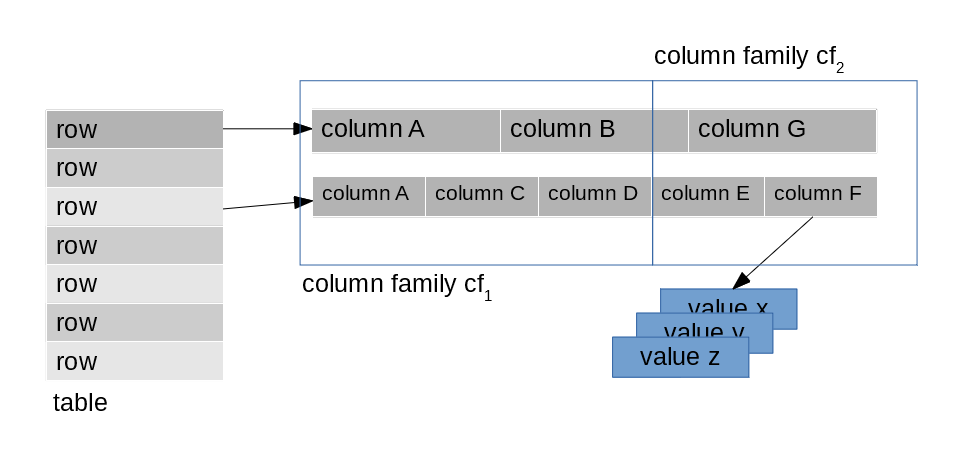
\includegraphics[width=1\textwidth]{images/hbaseTableStructure}
	\caption{structure of a HBase table}
	\label{hbase.fig1}
\end{figure}

The last paragraph already mentioned the storage of HBase. HBase is a so called column oriented database, therefore it does not store the records row by row but
column by column. Since HBase does not have a predefined schema but predefined column families for each table, it stores the values column family by column family.
Each column family is stored in a log structured merge tree, a data structure similar to the b+ trees that are used in traditional RDBMs. The log-structured merge tree
consists of multiple parts of which each is optimized for the storage medium it is stored on. When data is inserted into HBase, the new entry is inserted into a log file first.
After that, the new entry is inserted into an in-memory store. When the in-memory store reaches a certain threshold, it is flushed to the disk as a sorted list of key -> value.
This sorted lists are aranged like typical B-trees with an optimization for sequential disk access. During this process a background worker monitors the new files and merges files
that contain the same column family together after they reach a certain threshold to avoid jumps on the disk. \cite{hbase.george.2011} \cite{hbase.bertozzi.2012}

Although HBase's files are usually stored using the Hadoop File System, HBase itself distributes the data as well to allow for better hardware utilization. The data is distributed
in so called regions. Regions are ranges of rows that are stored together on one server. This must not be confused with the storage of column families: one file contains the data of one
column family, but one column family can be distributed over multiple files. Files that contain the data of the same rows are then stored together in one region. If a region reaches
a certain threshold, the region server splits the region into two regions. \cite{hbase.george.2011}
	
%!TEX root = ../dokumentation.tex

\section{Advantages and Disadvantages}
When evaluating the advantages and disadvantages of HBase it can be revealing to have a closer look at its features. According to \cite{hbase.achari.2015} HBase's characteristics can be named with the following key words: \textbf{sparse}, \textbf{distributed}, \textbf{multidimensional}, \textbf{map} and \textbf{sorted}. 

The word sparse seems to be a quite negative description for a database, at least in the german translation (dt.: dürftig). It sounds like HBase does not provide all of the important feautures a database should have. But actually the word sparse does not refer to the database itself but to the data stored within it. As described earlier the table schema can be absolutely flexible. The columns don't need to be the same in every row, two rows don't even need to be similar. For that reason there is no need to fill missing values with NULL to keep the schema consistent like it would be nessecary in relational databases. This saves storage space. Additionaly this structure has the advantage that columns can be added or removed at every moment of the database's lifetime. \cite{hbase.achari.2015}

Furthermore HBase is distributed to several nodes which can be either physically or virtually implemented. When using a physical implementation, the data is stored on several independent (physical) machines, \cite{hbase.wilson.2008} which are called \textit{Master Server} and \textit{Region Server}. Usually a cluster insists of several Region Servers which store the data \cite{hbase.vohra.2016} and at least one (up to nine) Master Servers which control the Region Servers within the cluster. \cite{hbase.apache.foundation.2017} This is HBase's auto failover which makes it reliable and protects against dataloss if one node in the cluster is failing \cite{hbase.wilson.2008} - on the condition that there has to be more than one Master Server, otherwise there’s the risk of a single point of failure if the Master Server fails. \cite{hbase.shriparv.2014}
Auto-sharding explains a bit more in detail how the data is stored on a Region Server. A region is the "basic unit of scalability and load balancing in HBase". And as already explained Chapter \ref{lblHBaseTechnologies} they simply contain contiguous ranges of rows. When these rows get to big for one Region Server they are split automatically by the system. This is called auto-sharding and permits the dristribution of data to different servers (Region Servers). This allows fast recovery after a server failed, as well as load fine-grained balancing because the regions can be moved between the Region Servers the way it is most suitable \cite{hbase.george.2011}

The terms multidimensional, map and sorted can be explained best in context. Map simply means the structure of key value pairs. Every value saved in the database has one specific key which consists of row key and timestamp among others. And these key value pairs are sorted alphabetically by key. This is important when designing the row key because at this point the administrator can ensure that relating values will be stored together within one region (e.g. two row keys of relating data: dhbw.2017.tinf14c and dhbw.2017.tinf14a). \cite{hbase.wilson.2008}
The conception of the key permits different versions for a value. Due to the timestamp whithin the key it is possible to overwrite an existing value without deleting it. Instead only the latest value is output on a table scan while the other versions are still available (see page \pageref{lblHBaseExample} Chapter \ref{lblHBaseExample}:  Update value). This is called multidimensional and gives the advantage of reproducing updates. \cite{hbase.achari.2015}

Additionally HBase has the advantage of the Apache Hadoop ecosystem with a lot of features especially for Big Data use cases, such as the MapReduce procedure for analytics. \cite{hbase.shriparv.2014}
The MapReduce procedure was just mentioned as an advantage but it also reveals a disadvantage. HBase does not handle JOINs like it is common in relational databases. Therefore the MapReduce layer provides a remedy. But as well it involves much more effort. A comprehensive knowledge about the Hadoop ecosystem would be necessary to use it effectively. And this fact actually applies to HBase in general. As it is not thought of being used as a standalone configuration the complexity of the Hadoop ecosystem is always there.
 As already mentioned when talking about sorted keys, it might also be a disadvantage that a row can only be indexed by its key whereas relational databases permit more options or using keys. \cite{hbase.shriparv.2014}

The HBase book \cite{hbase.apache.foundation.2017} gives advices when to use or when not to use the database. They definitively point out that it is not suitable for every problem. It is most important to have a huge amount of data. Huge amount in this context means hundreds of millions of rows, \textit{just} a few thousand or even million rows would not be enough to really get advantages from HBase. In this case it is suggested to stay with relational databases. This is for the reason that the cluster would not be made advantage of.
Then they stress that HBase is absolutely different from relational databases and most of the common features there are not available in HBase, such as data types, secondary indexes, transactions and advanced query languages. Therefore it is not possible to just migrate a relational database to HBase it is rather a complete redesign.
And finally they mention it is important to have enough hardware (minimum about five nodes) which is at least needed for the Hadoop filesystem. Indeed HBase can run standalone on a computer but this case should just be used for development cases. \cite{hbase.apache.foundation.2017}

Based on the investigation made for this chapter it seems like HBase provides more advantages than disadvantages. This should not be taken as a full fact but rather than a clue. When taking a decision for a NoSQL database it is advisable to compare these directly. This chapter mostly names advantages and disadvantages compared to relational databases. Therefore it might rather be helping to decide wheter a relational database or HBase are more suitable for the use case.


 	
%!TEX root = ../dokumentation.tex

\chapter{Example Project}
\label{lblHBaseExample}

This chapter's intention is to illustrate some of the technical facts discussed earlier. We used a standalone HBase setup on a virtual machine running Linux Ubuntu. For details on the installation process visit \href{www.hbase.apache.org/book.html\#quickstart}{www.hbase.apache.org/book.html\#quickstart}.

The following examples are executed with the HBase Shell, which is included in HBase's binaries. To start the shell execute 
\begin{lstlisting}[caption={start HBase shell},label=lst:hbas_shell]
	$ ./bin/hbase shell
\end{lstlisting}
in the HBase directory. 

\textbf{Create table student} \\
When creating a new table in HBase you need to specifiy the table's name as well as at least one column family. Additionally you can add parameter to specify the table setup. 
\begin{lstlisting}[caption={create table},label=lst:create_table]
	> create 'student', {NAME=>'personal',VERSIONS=>5}, 'school'
\end{lstlisting}
This command creates the table named \textit{student} with two column families \textit{personal} and \textit{school}. The column family personal is configured to store five versions of each column cell. This means that overwritten values are accessible until five overwrites. 

\textbf{Add row} \\
To insert a value you need to provide table name, row key, column family, column qualifier and value. 

\begin{lstlisting}[caption={insert values},label=lst:insert_values]
	> put 'student', 'Alexandra', 'personal:street', 'Schillerstrasse 31'
	> put 'student', 'Alexandra', 'personal:hair', 'blond'
\end{lstlisting}

The first line adds the value \textit{Schillerstraße 31} to the row \textit{Alexandra} in the table \textit{student}. The column family of this value is \textit{personal} and the column qualifier is \textit{street}. 

\textbf{Scan table} \\
When executing the following command all table entries are listed.
\begin{lstlisting}[caption={scan table},label=lst:scan_table]
	> scan 'student'
\end{lstlisting}

The output will look similar to this:

\begin{lstlisting}[caption={output of the table scan 1},label=lst:table_scan_output]
	ROW          COLUMN+CELL
	Alexandra    column=personal:hair, timestamp=1490775709059, value=blond
	Alexandra    column=personal:street, timestamp=1490775705439, value=Schillerstrasse 31
	1 row(s) in 0.0600 seconds
\end{lstlisting}

\textbf{Update value} \\
The value \textit{blond} should be updated to \textit{pink}.
\begin{lstlisting}[caption={update value},label=lst:update_value]
	> put 'student', 'Alexandra', 'personal:hair', 'pink'
\end{lstlisting}
Therfor again tablename, rowkey, column family and column qualifier are needed.
The output of scan table will look like this:
\begin{lstlisting}[caption={output of the table scan 2},label=lst:table_scan_output_2]
	ROW          COLUMN+CELL
	Alexandra    column=personal:hair, timestamp=1490776188067, value=pink
	Alexandra    column=personal:street, timestamp=1490775705439, value=Schillerstrasse 31
	1 row(s) in 0.0370 seconds
\end{lstlisting}

Only the most recent value is shown. To get more versions of an updated value a different command is needed.

\begin{lstlisting}[caption={get multiple versions},label=lst:get_multiple_versions]
	> get 'student', 'Alexandra', {COLUMN=>'personal',VERSIONS=>2}
\end{lstlisting}

\newpage
Now two versions of the values stored within column family \textit{personal} are displayed.
\begin{lstlisting}[caption={output of the table scan 3},label=lst:table_scan_output_3]
	COLUMN                                       CELL
	personal:hair        timestamp=1490776188067, value=pink
	personal:hair        timestamp=1490775709059, value=blond
	personal:street      timestamp=1490775705439, value=Schillerstrasse 31
	3 row(s) in 0.0880 seconds
\end{lstlisting}
\textbf{Note:} This is only possible if the column family is set to more than one version on table initiation. 

\textbf{Types} \\
To demonstate stat HBase does not enforce types, we updated a string value to an integer value.
\begin{lstlisting}[caption={put integer into cell},label=lst:put_integer]
	> put 'student', 'Alexandra', 'personal:hair', 3
\end{lstlisting}
HBase executes this without any (error) message. In fact everything is just stored as byte array.
The output looks like this:
\begin{lstlisting}[caption={output of the table scan 4},label=lst:table_scan_output_4]
	ROW          COLUMN+CELL
	Alexandra    column=personal:hair, timestamp=1490777492998, value=3
	Alexandra    column=personal:street, timestamp=1490775705439, value=Schillerstrasse 31
	1 row(s) in 0.0170 seconds
\end{lstlisting}

\textbf{Drop table} \\
To delete the table it must be disabled before it can be dropped.
\begin{lstlisting}[caption={drop table},label=lst:drop_table]
	> disable 'student'
	> drop 'student'
\end{lstlisting}	
%!TEX root = ../dokumentation.tex

\section{Conclusion}
HBase implements new column oriented concepts that Google introduced with BigTable. As a NoSQL database HBase does not need a fixed schema which makes it hard to use when the application is designed for RDBMS. Without the relational schema the key design in HBase is more important than in other databases. This on the one hand provides benefits but on the other hand also increases the effort of designing suitable keys. 

As a part of Apache Hadoop HBase supports clustering and distribution on many layers. HBase stores its data distributedly with HDFS while HBase's files are stored over multiple regions and servers. This and the underlying data structures improve the performance when inserting huge amount of data while still obtaining a high speed for analytical operations. Therfore, HBase is suitable for Big Data applications that deal with terabytes of data. 

Accordingly HBase is not suitable for relatively small amount of data. The costs of maintaining the Hadoop ecosystem and the additional effort on the key design do not generate substantial value for small applications.



\part{Key Value DB}
\chapter{Riak}
Riak is available in two versions. There is Riak TS for time series data and Riak KV. The chapter about Riak concentrates on Riak KV (further "Riak").
\section{Introduction into Riak}
The following chapter provides an introduction into Riak and its main features. 
\subsection{General Information}
Riak is a distributed key-value NoSQL database designed for high availability use cases. As long as the client can reach one Riak node the data is available. The reason is that data is saved across multiple servers. How the clustering works will be shown in the next chapter. \cite{Basho.06.04.2017}
\\
Riak is available for different operating systems, e.g. Ubuntu, CentOS or Mac OS X but not for Windows. The installation is straight-forward because you just have to download a package from the official website and install the package. \cite{Basho.06.04.2017}
\\ 
As data is saved across multiple servers even hardware or network failures can be handled by Riak. If you need more space for your data new servers can be added easily. By adding new servers the scalability is nearly linear which is very impressive. \cite{Basho.06.04.2017}
\\
Data is saved in buckets. A bucket in Riak can be compared with a table in a SQL-database. \cite{Basho.06.04.2017}
\\ 
Now if you have a look on the CAP-Theorem one can say that Riak definitely concentrates on "A" and "P" - Availability and Partition Tolerance. If your system needs high availability and you can not accept downtime Riak is probably the best solution. Another feature of Riak is its latency: since the CRUD-operations do not involve complex joins the requests are serviced promptly. \cite{Basho.06.04.2017}
\\
On the other hand if your system needs a high consistency of the data Riak is not the right choice. \cite{Basho.06.04.2017}
\subsection{Riak Clustering}
The high availability of Riak can only be achieved by the Riak clustering. The official website of Riak recommends that there should be at least five nodes in one cluster. A node is a server in production environment - during the development of the software there can be more than one node on a server. \cite{Basho.06.04.2017}
\\
All nodes have the same responsibility, this means there is no kind of master-node which has special tasks. \cite{Basho.06.04.2017}

The clustering is visible in the logo of Riak as well. There is one node and three lines to other nodes which symbolize the replication of data:
\begin{figure}[h!]
	\centering
	
\includegraphics[width=3.0in]{riak_logo.png}
	\caption[Riak Logo \protect\cite{Basho.06.04.2017}]{Riak Logo \protect\cite{Basho.06.04.2017}}
	\label{Riak Logo}
\end{figure}

\subsubsection{Automatic re-distribution of data}
When new servers are added or when machines are removed Riak automatically re-distributes the data with no downtime. Data is spread in the cluster until each node owns the same amount of data. This is why developers do not need to care about where the data is saved. Riak uses consistent hashing to distribute data evenly across the nodes in a cluster. Consistent hashing limits the reshuffling of keys when a hash-table structure is rebalanced. \cite{Basho.06.04.2017}
\subsubsection{Intelligent Replication}
Even if nodes fail the user should be able to read and write data. The replication scheme ensures the availability by setting a replication variable, that specifies the number of nodes on which a value will be replicated. The default number is three which means that each object is replicated three times. If Riak can access one node where the object is replicated it is available for the client. \cite{Basho.06.04.2017}
\\ 
The following picture describes the replication: 
\begin{figure}[h]
	\centering
	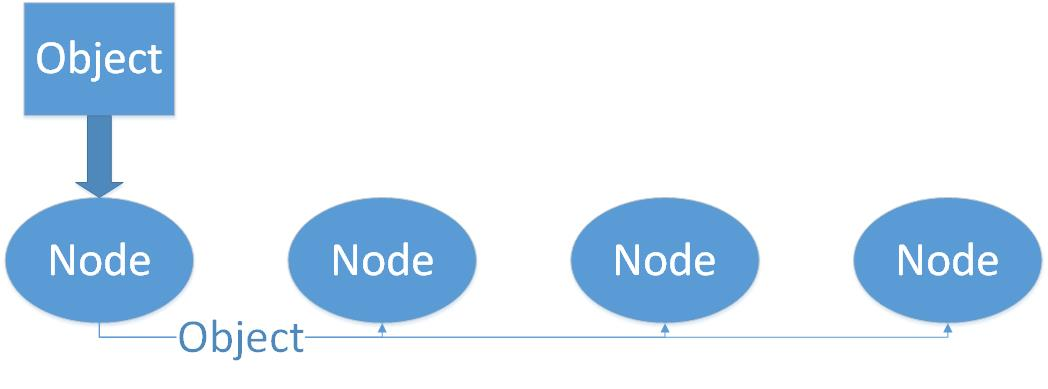
\includegraphics[width=3.0in]{riak_clustering.jpg}
	\caption{Riak Clustering}
	\label{Riak Clustering}
\end{figure}
\section{Open Source vs. Enterprise}

Basho provides five different versions of the Riak KV database letting the customers always find the perfect configuration for their purpose. The variants are named \textit{Open Source}, \textit{Developer}, \textit{Pro}, \textit{Enterprise} and \textit{Enterprise Plus}. Every configuration has a different composition of features. Figure \ref{fig:overview} shows a short overview of the versions and the related features.

\begin{figure}[ht]
	\centering
	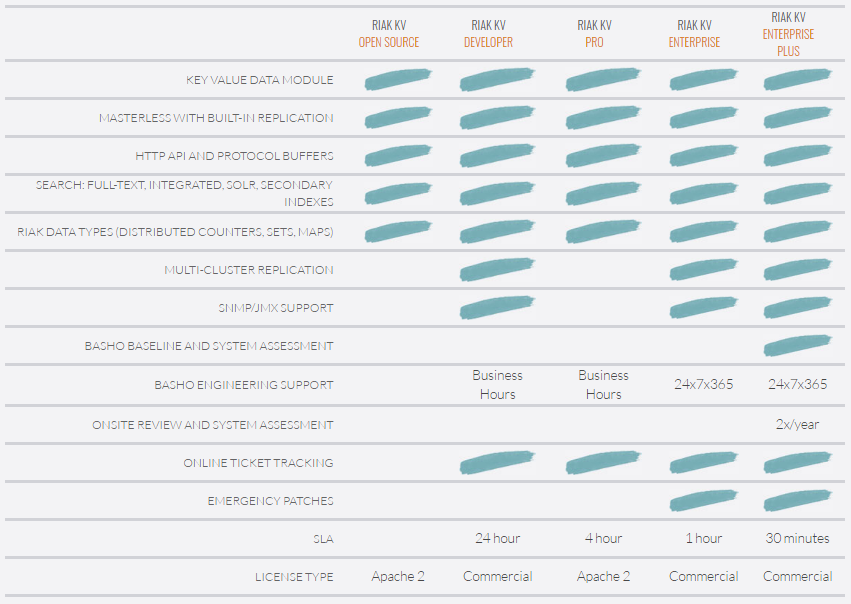
\includegraphics[width=\textwidth]{images/opensource_vs_commercial.png}
	\caption[Overview of different versions of Riak KV \protect\cite{Basho.01.04.2017}]{Overview of different versions of Riak KV \protect\cite{Basho.01.04.2017}}
	\label{fig:overview}
\end{figure}

In the following, every feature is individually viewed and explained in detail.

\newpage

\textbf{Key Value Data Module}\newline
Of course every configuration uses the key value data module developed by Basho.

\textbf{Masterless with Built-In Replication}\newline
All configurations are masterless with an integrated replication. This means that data is replicated automatically on multiple nodes so that the application remains available for both read and write operations. There is no single master and no single point of failure. This is the way the database achieves high availability. \cite{Basho.01.04.2017}

\textbf{HTTP API and Protocol Buffers}\newline
Every version works with a simple HTTP API and Protocol Buffers. Protocol Buffers is a method of serializing structured data and is especially useful for storing data. It is developed by Google. \cite{GoogleDevelopers.06.04.2017}

\textbf{Search}\newline
All implementations of the Riak KV support an integrated fulltext search and Apache Solr. Apache Solr is a popular open source enterprise search platform  built on Apache Lucene. This means with Apache Solr the user can search the whole database at once. \cite{TheApacheSoftwareFoundation.06.04.2017}

\textbf{Riak Data Types}\newline
Certainly all versions use the Riak data types which are \textit{Flags}, \textit{Registers}, \textit{Counters}, \textit{Sets} and \textit{Maps}. Flags are similar the same as Boolean, except the values are called \textit{enable} and \textit{disable}. Registers are essentially named binaries like Strings. Flags and Registers are no bucket-level Riak data types. They cannot be used on their own and have to be embedded in Maps. Counters keep track of increments or decrements. Sets are collections of unique binary values. Maps enable the creation of complex, custom data types because all other data types could be embedded. \cite{Basho.06.04.2017}

\textbf{Multi-Cluster Replication}\newline
This feature is only available for the commercial versions of Riak. The data clusters are replicated automatically in several data centers of the customer. If one cluster fails another one provides the necessary data. \cite{Basho.01.04.2017}

\textbf{SNMP / JMX Support}\newline
SNMP means \textit{Simple Network Management Protocol} and is a protocol for collecting and organizing information about managed devices on networks. \cite{L8ManeValidus.06.04.2017} JMX stands for \textit{Java Management Extensions} and is a Java technology that provides tools for managing and monitoring applications, devices and system objects. \cite{Bryanssm.06.04.2017} Customers that use a commercial configuration of Riak are able to implement these extensions and monitor their database.

\newpage

\textbf{Basho Baseline and System Assessment}\newline
This feature is obtainable just for customers of the Enterprise Plus package. An engineer of the Basho team reviews the whole configuration of the database via remote access before Riak is deployed. \cite{Basho.01.04.2017}


\textbf{Basho Engineering Support}\newline
The Basho Engineering Support is a simple support hotline. Since the Basho team only provides payed support, this offer is not available for the open source variant. The user has to have an account to contact the support team. \cite{Basho.01.04.2017}


\textbf{Onsite Review and System Assessment}\newline
That system assessment is nearly the same as the previous one. The only difference is that the assessment is not done via remote access, but a team of engineers come to the customers location and review the system onsite. \cite{Basho.01.04.2017}

\textbf{Online Ticket Tracking}\newline
The Online Ticket Tracking is a functionality of the account which is needed if you do not use the open source version. In combination with the ability to contact the support team, the user can see the current state of his support ticket. \cite{Basho.01.04.2017}

\textbf{Emergency Patches}\newline
If the customers of the Enterprise versions face a problem with their database, the Basho team provides a patch as soon as possible. \cite{Basho.01.04.2017}

\textbf{Service Level Agreements}\newline
The Service Level Agreements are between 24 hours and 30 minutes response time after a problem report was sent by the customer. Afterwards the engineering team provides a solution for the problem as soon as possible. \cite{Basho.01.04.2017} 

\textbf{License Type}\newline
The last point of this comparison is the license type. Riak KV Open Source and Riak KV Pro are available under the open source license Apache 2. The other three configurations use a commercial license. \cite{Basho.01.04.2017}

\newpage
\section{Advantages}
Since Riak is a distributed database there are different advantages making Riak special. Riak focuses on high availability, easy scalability and data safety. This is achieved through the distribution of the database across several nodes. \cite{Basho.01.04.2017}
The main advantages of the distributed approach are:
\begin{itemize}
	\item Installation
	\item Scalability
	\item Availability
	\item Interaction
	\item Error management
\end{itemize}
In the following subsections this concepts will be described in more detail. 
\subsection{Installation}
The installation of Riak is easy and straight forward. Riak is available for various Linux distributions and Mac OS X. There is an Dabian package for Ubuntu, delivered through bashos web page (HTTP://docs.Bashocom/riak/kv/2.2.2/downloads/). This package can be easily installed with Ubuntus package manager. After the setup you are ready to go. With the command \textit{"riak start"} a Riak cluster with one node and the standard settings is started. \cite{Basho.01.04.17c}
\subsection{Scalability}
Riak uses a distributed cluster approach built up of several nodes which makes it highly scalable. If there is a need for higher performance or stability there could be easily added several nodes to the cluster. This can be done even when the database is running. 
Before a node can be added to a cluster it needs to be started with the \textit{"riak start"} command. After the node is running it can be added to a cluster with the \textit{"riak cluster join"} command. \cite{Basho.01.04.17b}
\subsection{Availability}
A special feature of Riak is its high availability Riak uses a masterless system resulting in no single point of failure. If all nodes fail except one this last node will take all of the responsibilities of the other nodes. The cluster gets very slow, but it stays available and responsive.
\subsection{Interaction}
Another unique selling point of Riak is its native HTTP 1.1 API. This API is designed as RESTful Web service. Create, read, update and delete (CRUD) actions can be performed over the corresponding HTTP methods. This makes Riak a very flexible and handy database. 
Besides that Riak guarantees client support for common programming languages like Java, Ruby, Python, C\#, Node.js, PHP, Erlang and Go.  
\subsection{Error management}
If multiple clients can write concurrently and potentially to the same key it is very likely that errors could happen. Therefore Riak has to use an error management. There is an logical approach called vector clock which abstracts the states of a data set on an analogous clock to track the history of updates to a value. If the data is corrupted through conflict writes, it can be restored through this mechanism. 
\section{Disadvantages}
The distributed approach of Riak a very beneficial and useful as the previous section shows. But besides this advantages there are some downsides as well. Several nodes and the masterless concept lead to various problems like:
 \begin{itemize}
 	\item Inconsistency
 	\item Vector-clocks
 	\item No rollbacks
 \end{itemize}
 In the next subsections we will dig a little bit deeper in those problems. \cite{FHKoln.01.04.17}
 \subsection{Inconsistency}
 The main problem of highly-available, clustered systems like Riak is the validity of data sets. Due to the fact that there are no ACID transactions data sets can get inconsistent. There is no mechanism guaranteeing the transfer of a consistent state into another. This results in conflicting responses and anomalies which have to be handled.  
 \subsection{Vector-clocks}
 Although the error management concept of Riak is very reasoned the vector-clock system is leading to some difficulties. It is possible that Riak creates different values for an object on various nodes. These values are called siblings. This could lead to inconsistency and conflicts.
 \subsection{No rollbacks}
 Despite Riaks sophisticated error management system there is no way to completely restore a dataset. This is due to a missing rollback and commit mechanism. This means if you have done any change to the data it is irreversible.  
 \newpage
 \section{Use Cases}
 As you may have noticed, Riak is a quite special database solution. There are several use cases Riak is perfectly suited for. The first one described in here is session data. This means the usage of Riak for storing users and sessions into a Riak database. This data is usually used to save data about the applications connection with the user. Therefore it is very important to have this data highly available.
 Another common use case for Riak are chat and messenger applications. Traditional rational databases are not suited for the heterogeneous data messaging applications bring along. Therefore key value databases like Riak are more efficient way to save those data. Furthermore the highly-available, low-latency data architecture of Riak provides a good base for messaging apps which are always available.
 The next point is business continuity. This means applications which should not have a downtime of only several minutes. With Riak you can scale and maintain such applications even if the database is running. This is why Riak fits perfectly well to this use case.
 The last point described in this section is the usage of Riak for saving content and documents. This documents are highly unstructured because there are a huge amount of different data like pdf files, log files, emails, chat history, books, articles and videos. With Riak all of this data can be saved in a proper manner. There is no overload  as in a rational database. \cite{Basho.01.04.17}  
 
 To conclude with, Riak is used by several companies in the gaming, retail, telecommunications and transportation area as high available and scalable database. Well known companies which use Riak are Uber, Rovio, Best Buy, Xing and Symantec. \cite{Basho.01.04.17b}
 
 \newpage
\section{Conclusion}
All things considered one can say that the feature "CRUD"-Operations via REST is very useful but in newer versions \textbf{C}ross \textbf{O}rigin \textbf{R}esource \textbf{S}haring should be available since you can not send HTTP requests directly from an front-end to the database. 
\\
Furthermore Riak is a \textbf{distributed}, \textbf{scalable} and \textbf{fault-tolerant} NoSQL database. Use cases are mostly applications where high availability of data is the most important point. Another use case are applications with fast growing data as you can add new servers/nodes to your cluster and the data is replicated automatically. \cite{Basho.06.04.2017} 
\\
As already described in the chapter "Use Cases" Riak is especially useful for session data, documents, chat applications and business continuity as all of the use cases need a high availability of the data. \cite{Basho.06.04.2017}
\\
You should not use Riak if you expect the database to be always consistent since consistency is not possible. This is due to the CAP-Theorem where Riak concentrates on \textbf{A}vailability and \textbf{P}artition Tolerance.	

\part{Documentbased DB}
\section{Introduction to document based databases}
A possibility to realise NoSQL databases are document based databases. The structure of document based databases is like the structure of key-value databases. The big difference are the values which can be reached of the keys. At document based databases the value is a document. The document are collections of data and they exist in different structures. For example the data could be stored in XML or as a JSON object. But not every document is stored as a real document because a document is only a collection of data in the context of document based databases. \\
This formats have different possibilities to store the data but it is possible to store more then only one value in one document. An other part about document based databases is the structure of the documents. Every document in a database can have another structure. 
So it is possible to have a document which looks like the example in figure \ref{example1}.
\begin{mylisting}{\label{example1} Example of an document}
{"id":1,"age":25,"street":"examplestreet"}
\end{mylisting}
And another document which looks like the example in figure \ref{example2}. 
\begin{mylisting}{\label{example2} Example of an other document}
{"id":2,"user":"abc","country":"Germany"}
\end{mylisting}
%
But both can be stored in the same database also if they have not the same structure. 
The possibility of using JSON or XML as format gives this database a advantage when using it with some web applications. At web applications data are often stored in this formats and so it is a good possibility to save the data the same way in the database \parencite{DocDBIntro1,DocDBIntro2,DocDBIntro3}.
 
\chapter{CouchDB}
\section{Introduction}
This ebook was created in the context of a database Implementation lecture at the Cooperative University of Baden-Württemberg. This ebook should explain the base functionality of the document-oriented NoSQL database CouchDB. CouchDB's initial release was in year 2005. Nine years later CouchDB was released in stable version 2.0 \parencite{ApacheSoftwareFoundation.Branch}. CouchDB is developed in the programming language "Erlang" which was designed by	Joe Armstrong, Robert Virding and Mike Williams \parencite{ErlangWikipedia.22.03.2017}.\\
CouchDB is licensed with the Apache License 2.0. The initial idea of CouchDB was to developed a database which is easy to manage in the most common functions. So this was the reason why the developer creates a HTTP-based REST API \parencite{Anderson.2010.Buch} document storage model with a powerful query engine."\parencite{Anderson.2010.Buch} Based on this fact it is not possible to create SQL queries for data retrieval \parencite{Scheliga.2010}.
CouchDB stores the data in JSON-Format and the query language is Javascript \parencite{MarcelWolfKeineKommentare.2016}.
\\
\\

%This eBook is structured in three main section. The first section explains the document characteristics and the various design of documents. A big advantage of CouchDB is the HTTP-based REST API. Which this API it's possible manage the functionalities of CouchDB. The last section describes the base authentication mechanism, security issues and the administration of user%

%There is a theory which states that if ever anyone discovers exactly what the Universe is for and why it is here, it will instantly disappear and be replaced by something even more bizarre and inexplicable.
%There is another theory which states that this has already happened.
%\section{Document Structure}

Documents are CouchDB’s central data structure \parencite{Tutorialspoint, CouchDB.Guide}. 
Based on the fact that the CouchDB stores the content of the database not in tables another way is required. The data is stored in a specific form of documents.
%The creation of these documents can be done either with cURL utility provided by CouchDB or with Futon\cite{Tutorialspoint}.


%%%
\subsection{Document Characteristics}
A CouchDB server hosts named databases, which store documents \parencite{apache.docs.2.0}. As explained above, the documents are the place where the database content is stored. To access the data a way to retrieve the information from the documents is required. That is the reason why each document in CouchDB has a unique identifier ID \parencite{Brown.2012, Tutorialspoint}. The user can choose a specific ID that should be in the form of a string and based on the fact that we want to avoid collisions with twice used ID generally, the so-called Universally Unique Identifier (UUID) is used. In this way, the creation of duplicate IDs is prevented \parencite{Tutorialspoint}. \\
In addition CouchDB provides a RESTful HTTP API for database documents that can use these IDs to read, change and update documents \parencite{apache.docs.2.0}.
In the official apache docs, documents are described as the ``primary unit of data in CouchDB''  and they state out they can ``consist of any number of fields and attachments'' \parencite{apache.docs.2.0}. 
Furthermore do they include metadata values of varying types \parencite{apache.docs.2.0}. For example, text, number, boolean or lists \parencite{apache.docs.2.0}.
\newline


%%%%%%
%\begin{mdframed}[hidealllines=true,backgroundcolor=blue!20]
%\textcolor{red}{evtl Überflüssig}
%Documents are self-contained units of data. You might have heard the term record to describe something similar. Your data is usually made up of small native types such %as integers and strings. Documents are the first level of abstraction over these native types. They provide some structure and logically group the primitive data. The %height of a person might be encoded as an integer (176), but this integer is usually part of a larger structure that contains a label ("height": 176) and related data %(${"name":"Chris", "height": 176}$).\cite{CouchDB.Guide}
%
%The CouchDB document update model is lockless and optimistic. Document edits are made by client applications loading documents, applying changes, and saving them back to %the database. If another client editing the same document saves their changes first, the client gets an edit conflict error on save. To resolve the update conflict, the %latest document version can be opened, the edits reapplied and the update tried again.\cite{apache.docs.2.0}
%Document updates (add, edit, delete) are all or nothing, either succeeding entirely or failing completely. The database never contains partially saved or edited %documents.\cite{apache.docs.2.0}
%
%Documents differ subtly from garden-variety objects in that they usually have authors and CRUD operations (create, read, update, delete). Document-based software (like %the word processors and spreadsheets of yore) builds its storage model around saving documents so that authors get back what they created. Similarly, in a CouchDB %application you may find yourself giving greater leeway to the presentation layer. If, instead of adding timestamps to your data in a controller, you allow the user to %control them, you get draft status and the ability to publish articles in the future for free (by viewing published documents using an endkey of %now).\cite{CouchDB.Guide}
%
%Say your users can comment on the item (“lovely book”); you have the option to store the comments as an array, on the item document. This makes it trivial to find the %item’s comments, but, as they say, “it doesn’t scale.” A popular item could have tens of comments, or even hundreds or more.\cite{CouchDB.Guide}
%
%Instead of storing a list on the item document, in this case it may be better to model comments into a collection of documents. There are patterns for accessing %collections, which CouchDB makes easy. You likely want to show only 10 or 20 at a time and provide previous and next links. By handling comments as individual entities, %you can group them with views. A group could be the entire collection or slices of 10 or 20, sorted by the item they apply to so that it’s easy to grab the set you %need.\cite{CouchDB.Guide}
%
%A rule of thumb: break up into documents everything that you will be handling separately in your application. Items are single, and comments are single, but you don’t %need to break them into smaller pieces. \cite{CouchDB.Guide}
%\end{mdframed}
%%%%



\subsection{Design Documents}
Design documents are a special type of CouchDB document and beside the core document storage it is probably the most important component of the CouchDB database \parencite{CouchDB.Guide,Brown.2012}. These documents contain the application code or in other words, they contain the database logic about the document \parencite{CouchDB.Guide,Brown.2012}. \\
``Think of the design document as the glue that turns each of your documents into the format or structure that you need for your application.'' \parencite{Brown.2012}
This quote shows the importance of design documents.
%The key to all of these different types of information, %and many others, is the design document. Aside from the %core document storage, the design document is probably %the most important component of your CouchDB database. %Design documents contain all of the database logic about %the document you are storing. Think of the design %document as the glue that turns each of your documents %into the format or structure that you need for your %application.
%\cite{Brown.2012}
To understand the structure of design documents it is necessary to understand what design documents provide. \\
The following paragraphs explain the purpose of: 
\begin{itemize}
    \item Views
    \item Shows
    \item Lists
    \item Validations
    \item Update handlers
    \item Filters
\end{itemize}
\textbf{Views} \\
Functions that create lists of documents data are called views. Therefore, they take and process the information inside documents to create lists, that are even search-able. The process to create views is incredibly simple and very powerful because in fact, the user does not need to know the document ID \parencite{Brown.2012}. In other words, views are an easy way to organise and group documents in a way that help to understand the meaning of the documents content \parencite{CouchDB.Guide}. The purpose of the view is also described as the collection of documents \parencite{Brown.2012}. \\
\newline
%%%%
%Views are the primary tool used for querying and %reporting on CouchDB databases.\cite{apache.docs.2.0}
%%%%
\textbf{Shows} \\
To convert a document to another format, a show function is needed. Usually, the most useful format is HTML, although the user can select any format, including JSON or XML if these formats suit their application better. One reason to use a format changing function is that in that way it is possible to simplify the document's JSON content to a reduced format \parencite{Brown.2012}.\\
\newline
%Show functions are used to represent documents in %various formats, commonly as HTML pages with nice %formatting. They can also be used to run server-side %functions without requiring a pre-existing %document.\cite{apache.docs.2.0}
\textbf{Lists} \\
A list is to a view as a show is to a single document. The list function is used to format the view as an HTML table, or a page of information or as XML of your document collection. In this way, a list transforms the entire content of one view into another format \parencite{Brown.2012}. CouchDB list functions allow you to create the output of views in any format \parencite{CouchDB.Guide}.
Here’s an example \parencite{CouchDB.Guide} design document that contains one list function:
\begin{mylisting}{Example List Function \parencite{CouchDB.Guide}}
{
  "_id" : "_design/foo",
  "_rev" : "1-67at7bg",
  "lists" : {
    "zoom" : "function() { return 'zoom!' }",
  }
}
\end{mylisting} \\
%\begin{mdframed}[hidealllines=true,backgroundcolor=blue!20]
%\begin{lstlisting}[basicstyle=\ttfamily\small,breaklines=true,caption=blabla, label=amb]
%{
%  "_id" : "_design/foo",
%  "_rev" : "1-67at7bg",
%  "lists" : {
%    "zoom" : "function() { return 'zoom!' }",
%  }
%}
%
%\end{lstlisting}
%\end{mdframed} \\
%%%
%While Show Functions are used to customize document %presentation, List Functions are used for the same %purpose, but on View Functions %results.\cite{apache.docs.2.0}
%%%%
\textbf{Document Validation} \\
To maintain consistency in the CouchDB we need so-called validation functions. ``Often in document-based software, the client application edits and manipulates the data, saving it back \parencite{CouchDB.Guide}.'' Right after the saving of a new document into CouchDB the validation function is called. This function can either check or even reformat the incoming document to meet your requirements and standards for different documents \parencite{Brown.2012}. With Validation functions, the user does not have to worry about data causing errors in the DB \parencite{CouchDB.Guide}. \\
\newline
\textbf{Update Handlers}\\
If the user wants to execute an action on a specific document after updating it he or she have to use update handlers. Unlike document validation are these handlers explicitly called. As an example can these handlers be used to increment values in a document or add and update timestamps \parencite{Brown.2012}. \\ 
%Unlike document validation, update handlers are explicitly called, but they can be used to make changes to a document within the server without having to retrieve the document, change it, and save %it back (as would be required for a client process). 
\newline
\textbf{Filters}\\
The example of storing information about a CD and DVD collection explains the usage of filters very well.
If the user stores information about a CD and DVD collection in a single database, he or she may wants to exchange only the CD records with another database \parencite{Brown.2012}. In some use cases, it might be useful to filter the content of the database. These use cases could be, for example, exchanging information between CouchDB databases or using replication \parencite{Brown.2012}. If filter functions are called, it probes the list of supplied documents from the replication and then either returns the document or null \parencite{Brown.2012}. \\
%In addition, it is notable that any database can have zero or more design documents\cite{Brown.2012}.

%%%
%Filter functions mostly act like Show Functions and List %Functions: they format, or filter the changes %feed.\cite{apache.docs.2.0}
%%%

\subsection{JSON Document Format}
CouchDB uses JavaScript Object Notation (JSON) for data storage \parencite{Anderson.2010.Buch}.
%%Appendixquelle
The author Tim Juravich describe JSON as the ``strange markup of the document'' \parencite{Juravich2012}. ``JSON is a lightweight data-interchange format based on JavaScript syntax and is extremely portable \parencite{Juravich2012}.''
%The basic format of the design document is a JSON document with a field for each of the major content types (view, list, shows)\cite{Brown.2012}.
%Depending on the type, the definition then contains one or more further definitions\cite{Brown.2012}.
\newpage
\begin{mylisting}{Example JSON Document based on \parencite{Brown.2012}}
{
    "language": "javascript",
    "views": {
        "all": {
            "map": "function(doc) { emit(doc.title, doc) }",
        },
        "by_title": {
            "map": "function(doc) { if (doc.title != null) emit(doc.title, doc) }",
        },
        "by_keyword": {
            "map": "function(doc) { for(i=0;i<doc.keywords.lenghth();i++) { emit(doc.keywords[i], doc); } }",
        },
    },
    "shows": {
        "recipe": "function(doc, req) { return '<h1>' + doc.title + '</h1>' }"
}
\end{mylisting}
%%
%%
%%
%\begin{mdframed}[hidealllines=true,backgroundcolor=blu%e!20]
%\begin{lstlisting}[basicstyle=\ttfamily\small,breaklin%es=true]
%{
%    "language": "javascript",
%    "views": {
%        "all": {
%            "map": "function(doc) { emit(doc.title, %doc) }",
%        },
%        "by_title": {
%            "map": "function(doc) { if (doc.title != %null) emit(doc.title, doc) }",
%        },
%        "by_keyword": {
%            "map": "function(doc) { %for(i=0;i<doc.keywords.lenghth();i++) { %emit(doc.keywords[i], doc); } }",
%        },
%    },
%    "shows": {
%        "recipe": "function(doc, req) { return '<h1>' %+ doc.title + '</h1>' }"
%}
%\end{lstlisting}
%\end{mdframed} \\
%%%%%
The example in figure 1.2 provides a simple design document that defines three views and one single show \parencite{Brown.2012}. The syntax of JSON should be pretty self-explanatory. Curly braces wrap objects. Every Object is key/value lists and the keys are strings, which are wrapped in double quotes. A value can be a string, an integer, an object, or an array \parencite{CouchDB.Guide}. Keys and values are separated by a colon and multiple keys and values by comma \parencite{CouchDB.Guide}. \\
%One of the best bits about JSON is that it’s easy to read and write by hand, much more so than something like XML\cite{Anderson.2010}. We can parse it naturally with %JavaScript because it shares part of the same syntax\cite{Anderson.2010}. This really comes in handy when we’re building dynamic web applications and we want to fetch %some data from the server\cite{Anderson.2010}.
%Here’s a sample JSON document:
%\begin{mdframed}[hidealllines=true,backgroundcolor=blue!20]
%\begin{lstlisting}[basicstyle=\ttfamily\small,breaklines=true]
%{
%    "Subject": "I like Plankton",
%    "Author": "Rusty",
%    "PostedDate": "2006-08-15T17:30:12-04:00",
%    "Tags": [
%        "plankton",
%        "baseball",
%        "decisions"
%    ],
%    "Body": "I decided today that I don't like baseball. I like plankton."
%}
%\end{lstlisting}
%\end{mdframed} \\
In other words, the general structure is based around key/value pairs and lists of things \parencite{Anderson.2010.Buch}.

%\subsection{Modeling Documents}

%\subsection{Query Server}

%\subsection{Applications = Documents}

%\subsection{Example Design Document}

%Example:

%EXAMPLE OF A COUCHDB DOCUMENT
%Let's take a look at an example of what a CouchDB document might look like for a blog post:
%
%${
%"_id": "431f956fa44b3629ba924eab05000553",
%"_rev": "1-c46916a8efe63fb8fec6d097007bd1c6",
%"title": "Why I like Chicken",
%"author": "Tim Juravich",
%"tags": [
%"Chicken",
%"Grilled",
%"Tasty"
%],
%"body": "I like chicken, especially when it's grilled."
%}$
%\cite{Juravich2012}

%\newpage
%\section{REST http API}


To control and get access to a CouchDB instance it is possible to use a REST API. This API is the first selection of managing the database but it is also possible to use Fauxton which is an administration interface for CouchDB. This chapter will introduce the REST API and will give an overview about the main functionalities. First of all some basics will be explained after that the sections of the API will be introduced. The different sections would be: The server part, the database part, the document part and the replication part.

\subsection{Basics}

The REST API is used over standard http or https methods. The CouchDB API doesn’t support all possible HTTP requests methods for example the “PATCH” method isn’t supported. Possible methods are: GET, HEAD, POST, PUT, DELETE and COPY. For example the GET method is used to get a specific item of the database and the PUT method allows to create a new object in the database. The root URI to send a request would be \url{http://www.domain.tld:portnumber/}  at the default configuration. But also many other URIs with the root URI at the beginning are existing for every single operation \cite{CouchDBRestRFCPatch, CouchDBRestBasic}. \\
To get or send the needed data a standard data structure has to be defined. The CouchDB REST API uses the JavaScript Object Notation (JSON) to structure the data. The motivation for JSON is “because it is the simplest and easiest solution for working with data within a web browser, as JSON structures can be evaluated and used as JavaScript objects within the web browser environment. JSON also integrates with the server-side JavaScript used within CouchDB.“ \cite{CouchDBRestJson}  \\
For this reason it is also recommend to mostly set the header of the http request at “accept” to “application/json” instead something special is needed. One additional thing to know is the fact that the header “Content-Type” should be “text/plain” even if the information is saved at the JSON format. If the json from the user was incorrect for example if it was not formatted correctly the response of the API would be the HTTP Status Code 500. In addition to this Status Code the API also uses other standard HTTP Status Codes like 200, 201, 400, 404 or others. But not all codes are supported but the meaning of all used codes is documented\cite{CouchDBRestBasic}.

\subsection{The Server Part}
 
The server part of the REST API starts at the root URI \url{http://www.domain.tld:portnumber/}. For example a get request to this URI gives a response with information about the status of the database server. 
Generally the server part has different URIs which can be used to configure the server or to get specific information. For example it is possible to call \url{http://www.domain.tld:portnumber/_all_dbs} which returns all created databases at the server.
It would be look like this json string: [“testdb","testdb1","testdb2"]. 
If no database exists it would give an empty JSON array: []. 
Finally the server part concludes all necessary information about the server and also gives some options which are helpful for the administration part of the database server \cite{CouchDBRestServer}.

\subsection{The Database Part}
\label{subsec:TheDatabasePart-1}

The database part of the REST API concludes all operations which can be used for one database. It starts with creating a database and goes over to add entries and configure the security options of a database.
An example to create a database would be following PUT request at the URI:
\url{http://localhost:5984/<databasename>/_security}. \\
Another example would be to configure the security settings of the database “testdb”:
First the current settings would be requested over GET  \url{http://localhost:5984/testdb/_security} with the response which can be seen following: 
\begin{lstlisting}[frame=single, caption= Example security response]
{
    {
        "admins":{"names":["admin"],
        "roles":["adminstrators"]},
        
        "members":{"names":["user"],
        "roles":["tester"]},
        "ok":true
    }
}
\end{lstlisting} 
\newpage 
After that a PUT request to the same URI with the following body is send:
\begin{lstlisting}[frame=single, caption= Put request body]
{
    {
        "admins":{"names":["admin","admin2"],
        "roles":["adminstrators"]},
        "members":{"names":["user"],
        "roles":["tester"]},
        "ok":true
    } 
}
\end{lstlisting} \\
The request returns only a short answer from the REST API: 
\begin{quote}{"ok":true} \end{quote}
A second GET request to the same URI returns the string which can be seen following:
\begin{lstlisting}[frame=single, caption=  Get response]
{
    {
        "admins":{"names":["admin","admin2"],
        "roles":["adminstrators"]},
        "members":{"names":["user"],
        "roles":["tester"]},
        "ok":true
    }
}

\end{lstlisting}
All URIs which belongs to the database part of the API are available under  \url{http://localhost:5984/<databasename>/<command>}. So only the right database name and the right command has to be appended to the root URI \parencite{CouchDBRestDatabases}.

\subsection{The Document Part}

The document structure is a central element of the database and it has also an own part in the API. This part manages the CRUD (create, read, update, delete) operations to the documents which belongs to one database. The design of the REST API gives the possibility to manage more then one database so it is necessary to have the possibility to select the database first and then select the document. \\
In the chapter \nameref{subsec:TheDatabasePart-1} the database part is presented with the \url{http://localhost:5984/<databasename>} path. This path is going to be expanded to \url{http://localhost:5984/<databasename>/<documentid>}. This basic path could be used for different options which can be used to the document. This options are selected about the HTTP request methods. For example PUT is used to create a new document with information in JSON string which is stored in the request body. Other available methods are: HEAD, GET, DELETE and COPY.  \\
All necessary options to the documents are realized with this one URI without the part of the attachments. CouchDB has the possibility to add attachments to a document. The management of this attachments over the REST API is realised on the same way like the management of the documents. The only difference is the missing HTTP COPY method and a different path. For the attachments the path \url{http://localhost:5984/<databasename>/<documentid>/<attachmentname>} is used. About this path all operations can be executed \cite{CouchDBRestDocuments}.

\subsection{The Replication Part}

CouchDB also supports the replication between two databases. This option is managed by some settings which can be managed by the URI \url{http://localhost:5984/_replicate}. With this URI is only one single replication triggered it is not like a background job which is executed every X minutes. The interesting part of this URI is the fact that is not a correct RESTful API method. The RESTful architecture has one principle which means that every request gives a representation of an object. The call for the replication is only the call of a procedure which is located on the server or on another remote location \cite{CouchDBRestReplication}.

\subsection{Conclusion}

Finally the REST API of CouchDB gives the possibility to do all operations which are possible about an graphic user interface also about the REST API and the HTTP protocol. But also it should be noticed that not all methods are complete RESTful and they are mixed with methods which comply with the REST architecture. 
The documentation argue with the fact that they want to use the optimal technique for all events and so they decide to mix both ways together to give the user a better experience. 


%\newpage
%\section{Security}

Storing sensitive data today requires a high standard of IT security. If databases store personal data or business secrets it is necessary to protect these data against loss, destruction and theft. For this reason the  database architects  should be informed about the actual security mechanism, authentication mechanisms and about existing security gaps. This chapter describe the base authentication mechanisms, security issues and the administration of users.

\subsection{User Authentication}
After the first installation of CouchDB every user disposes automatically over privileges of an administrator. Every user can create database or change system properties. This very big security gap is also known as "Admin Party". Since version 0.11 it is possible to differ between three user roles \\ \cite{ApacheSoftwareFoundation.2013.SecurityFeatures}:
\begin{enumerate}
\item Server administrator \\
The user role of a server administrator disposes of all privileges. They have reading access and writing access to all databases stored on the CouchDB server and can change all server settings \cite{Anderson.2010.Buch}.
\item Database administrator

The database administrator disposes of reading access and writing access of one specific database. This user role have the privileges to create, edit, delete documents but "they can not create and neither delete [other] databases." \cite{ApacheSoftwareFoundation.2013.SecurityFeatures}
Additional they can create new database members and database admins for these specific database.
\item Database members \\
The database members have reading access to all documents but they have only writing access to 'normal documents'. Especially they can not change design documents.
\end{enumerate}
\textbf{Creating server administrator}\\
There are two technical capabilities to create a new server administrator. The first possibility is to change the \textit{local.ini} file \\ \cite{ApacheSoftwareFoundation.2013.AdminAccount}:
\begin{lstlisting}{frame=single, caption=Example Create new Server Administrator with local.in File \protect\cite{ApacheSoftwareFoundation.2013.AdminAccount}}
[admins]
username = password
\end{lstlisting}

Currently every admin has the possibility to read these plain-text password. This situation is a very big security gab. Only after restart CouchDB the password will be encoded with a hash. This hash will be create within three steps \cite{Anderson.2010.Buch}:
\begin{enumerate}
\item creates a new 128-bit [Universally Unique Identifier] (random numbers with low collision probability) = \textbf{salt} \cite{Anderson.2010.Buch}
\item "Creates a sha1 hash of the concatenation of the bytes of the plain-text password and the salt (sha1(password + textbf{salt}))" \\ \cite{Anderson.2010.Buch}
\item "Prefixes the result with -hashed- and appends textbf{salt}" \\ \cite{Anderson.2010.Buch}
\end{enumerate}
After restart CouchDB the \textit{local.ini} looks like:
\begin{lstlisting}{frame=single, caption=Example Create new Server Administrator with local.ini File \protect\cite{ApacheSoftwareFoundation.2013.AdminAccount}}
[admins]
username = -hashed-207b1b4f8434dc60429672c0c2ba3aae61568d6c,96406178a0718239acb72cb4e8f2e66e
\end{lstlisting}
But it also possible to create a server administrator with the provided API (for further information please see chapter 1.4.3 "The Database Part"): \\ \cite{Anderson.2010.Buch}
\begin{lstlisting}{frame=single, caption=Example Create new Server Administrator with REST API \protect\cite{Anderson.2010.Buch}}
curl -X PUT \$HOST/\_config/admins/username -d '"password"'
\end{lstlisting} 

Until now it is only possible to create a new databases after you entered the administrator password. \\
\\
\textbf{Creating database administrator and database members}
\\
To create a database administrator or a simple database member it is necessary to change the security object of the selected database. These object is located under \textit{\slash db\_name\slash\_security} \\ \cite{ApacheSoftwareFoundation.2013.SecurityFeatures}.
The data in these object is in JSON format \cite{ApacheSoftwareFoundation.2013.SecurityFeatures}:
\begin{lstlisting}{frame=single, caption=Example Create new Database Members and Database Administrator \protect\cite{ApacheSoftwareFoundation.2013.SecurityFeatures}}
{
  "admins" : {
     "names" : ["ines", "tobi"],
     "roles" : ["boss"]
   },
   "members" : {
     "names" : ["leon"],
     "roles" : ["producer", "consumer"]
   }
}
\end{lstlisting}

\textbf{If a database have no database users every user can change regular documents!}
CouchDB stores data of the single users in an user authentication database named (\_\textbackslash users). Every user have a separate document. In this document it is possible to save the properties of every user for example id, name or user roles.The property "type" can only substituted with the key "user". An example user definition in such a document is shown in the following graphic: \cite{ApacheSoftwareFoundation.2013.SecurityFeatures}:
\begin{lstlisting}{frame=single, caption=Example User Definition \protect\cite{ApacheSoftwareFoundation.2013.SecurityFeatures}}
{
 "\_id":"org.couchdb.user:ines",
 "type":"user",
 "name":"ines",
 "roles":["guest"],
 "password\_sha":"fe95df1ca59a9b567bdca5cbaf8412abd6e06121",
 "salt":"4e170ffeb6f34daecfd814dfb4001a73"
}
\end{lstlisting} 

\subsection{Cookie Authentication}
The standard user authentication with user name and password shows a increasingly security gap. Therefore, CouchDB offers the possibility of user authentication with Cookies. By the use of Cookies users can be authenticate without filling user-related data in permanent opened password dialogues. 
CouchDB offers the possibility to use Proxy or implement particular authentication modules to sync or authenticate user data with existing LDAP systems or Active Directory \cite{Anderson.2010.Buch}.

\subsection{Validation Function}
To be able to guarantee the consistency of the data in a database system, it is helpful to provide rules directives. Afterwards every document must fulfill these requirements. For example, it is possible to define directives which ensures that the field "name" may not bee empty. If this field will be empty an error message will be shown. \cite{Scheliga.2010}.

\begin{lstlisting}{frame=single, caption=Example Validation Function \protect\cite{Scheliga.2010}}
{
    \_id: "\_design/designdoc",
    validate\_doc\_update: "function(newDoc, oldDoc, userCtx) {
    if(newDoc.name === undefined) {
    throw {forbidden: 'Document must have a name.'};
    }}"
}
\end{lstlistings}

The deposited validation directives launch automatically if a new document created or an existing document changed. Every validation directives can include an arbitrarily number of these rules. However every design document can only deposit one validation function \cite{Scheliga.2010}.



%\section{Conclusion}
In conclusion, this book explains the background to understand the concept of the document-based database CouchDB. The provided information give a deep inside on the document structure, the REST http API and security aspects the user gets in contact by using CouchDB.
In addition to the provides overview, there are some advantages and some disadvantages of using CouchDB that are notable.\\
\newline
On the one hand, big advantages of CouchDB are the scalability and fast read and write operations. 
More features that can be described as advantages are for example the synchronisation, offline usage and the support for mobile devices. CouchDB has the ability to synchronise between multiple databases and in addition the offline functionality provide the function that data on the device can be manipulated and synced later, when the device get a connection to the main database \cite{MoronyJosh}. 

%Synchronising two or more databases can be astoundingly %difficult, and in order to provide offline functionality %in an application, we need to provide local data to the %user that can be read and modified, and then later synced %back to the main database or databases when a network %connection becomes available.
%Built for Offline
%CouchDB can replicate to devices (like smartphones) that %can go offline and handle data sync for you when the %device is back online.
%
%Distributed Architecture with Replication
%CouchDB was designed with bi-direction replication (or %synchronization) and off-line operation in mind. That %means multiple replicas can have their own copies of the %same data, modify it, and then sync those changes at a %later time.
Another important advantage is the way the document storage is implemented. Based on the fact that everything is stored as documents and there is no pre-defined schema the way how the datasets are designed is up to the user. This creates a lot of flexibility for data storage, but it also has its downsides and it can be difficult to learn because there is no \textit{100\%} correct way to store the data \cite{MoronyJosh}. 
%Unlike a relational database where we need to describe what the structure of our data is before we insert it (a schema), and can only insert data that matches that schema, with CouchDB you can store whatever kind of data you want, whenever you want. This doesn’t mean that there is no structure to a CouchDB database, it is critically important that you add data in a way that makes sense and will perform well for your application. This creates a lot of flexibility for data storage, but it also has its downsides and it can be quite hard to learn because there is no “100percent correct” way to store the data, and in many cases, it’s better to do things you will probably have learned to avoid like duplicating data.\cite{MoronyJosh}
%I'd say the following are some of CouchDB's advantages:
%
%the document model
%simple REST API
%changes feed
%relatively easy to set up multiple nodes but with some %caveats.
%I like the document model because it matches up with most %of the real world uses I think a lot of us have. It's %easy to serialise objects to JSON, store them and then %retrieve and deserialise when we need them back. With a %column store, like Cassandra, you'd have some of the %schema inflexibility that you get with a relational %database.
%
%As a document store, rather than a pure key-value store, %CouchDB also lets you index and query the contents of %your documents, rather than just pulling them out %wholesale. So, if indexing/querying the contents of %documents is important then it'll suit you better than %something like Riak.
%
%Against MongoDB, I think the main advantage is that %CouchDB is architected in a way that makes it easier to %grow a cluster. I mean, this depends on your precise %needs. For example, with CouchDB you can add more and %more nodes relatively easily and set up replication %between them. That can be great for availability but %you're replicating the same full data set on each node, %so it might be so great for really large data sets.
%
%You might want to look at CouchDB's spritual descendant, %Couchbase. Couchbase is also open source and was created %by many of the same team. It uses hash-based partitioning %and clustering, similar to Cassandra, but retains the %document model. So, it's pretty much linearly scalable %but lets your work with schema-unenforced JSON docs.
%
%\cite{RevellMatthew}
%Document Storage
%CouchDB stores data as "documents", as one or more %field/value pairs expressed as JSON. Field values can be %simple things like strings, numbers, or dates; but %ordered lists and associative arrays can also be used. %Every document in a CouchDB database has a unique id and %there is no required document schema.
%
%
%
%Map/Reduce Views and Indexes
%The stored data is structured using views. In CouchDB, %each view is constructed by a JavaScript function that %acts as the Map half of a map/reduce operation. The %function takes a document and transforms it into a single %value that it returns. CouchDB can index views and keep %those indexes updated as documents are added, removed, or %updated.
Furthermore, CouchDB provide a simple REST API where all items have a unique URI that gets exposed via HTTP.
%It uses the HTTP methods POST, GET, PUT and DELETE for the four basic CRUD (Create, Read, Update, Delete) operations on all resources.
In addition, the build-in administration interface Futon that is accessible via Web provide a easy way to interact with the database and is with the REST API feature one of the most important advantages. 

%%
%%%%%%%%
%Data in CouchDB, like in many (but not all) NoSQL %databases, is stored as documents and there is no %pre-defined schema. Unlike a relational database where we %need to describe what the structure of our data is before %we insert it (a schema), and can only insert data that %matches that schema, with CouchDB you can store whatever %kind of data you want, whenever you want. This doesn’t %mean that there is no structure to a CouchDB database, it %is critically important that you add data in a way that %makes sense and will perform well for your application. %This creates a lot of flexibility for data storage, but %it also has its downsides and it can be quite hard to %learn because there is no “100percent correct” way to %store the data, and in many cases, it’s better to do %things you will probably have learned to avoid like %duplicating data.\cite{MoronyJosh}
%%%
\newline
On the other hand, some drawbacks are worth mentionable.
%Eventual Consistency
CouchDB guarantees eventual consistency to be able to provide both availability and partition tolerance. In detail, this implies two write and read operations in the same time frame will cause the problem, that the update will not necessarily be see-able \cite{EminGunSirer}.
It is likely that some use-cases do not work with this issue. For example, selling concert tickets, would not work with this model \cite{EminGunSirer}. \\
%%%CONS
%Cassandra and Couch are eventually consistent, which %implies that a client might perform an update, receive an %acknowledgment, yet another client performing a read will %not necessarily see that update. Your applications may or %may not be able to deal with this kind of behaviour in the %data store. Many applications, such as selling concert %tickets, would not work with this model. Others, such as %shopping carts, could perhaps work ok, assuming that %their users can clear up occasional %inconsistencies.\cite{EminGunSirer}
%Other features include document-level ACID semantics with %eventual consistency, (incremental) MapReduce, and %(incremental) replication. One of CouchDB's distinguishing %features is multi-master replication, which allows it to %scale across machines to build high-performance systems.
%
%
%
%After the installation of CouchDB it is very important to %check the several security functions. The most important %point is to create a valid user structure which differs %between the three user roles:
%\begin{enumerate}
%\item Server Administrator
%\item Database administrator
%\item Database members
%\end{enumerate}
%
%%%%%
%
%
%
Remarkable is that only a few big projects are published which use CouchDB. For example, the platform readwrite published that "the Compact Muon Solenoid Experiment (CMS) at CERN (The European Organization for Nuclear Research) will deploy the NoSQL database CouchDB into production this summer"\cite{KLINTFINLEY.2010}. In addition, CouchDB is also used by CloudWork\cite{BrunoPedro.2013}. \\
Resting upon the pros and cons it is noticeable that every use-case for the database has to be conceptualised to proof either CouchDB is the right solution or not. Thereby, this ebook has the purpose to contribute strongly to the overall course ebook about NoSQL databases. 



\chapter{MongoDB}
This chapter guides you through the features of MongoDB. Whereby we go through what is MongoDB in general, Data model and CRUD Principles. Thereafter we check through the Use-Cases of MongoDB and performance and limitations. Additionally, we get a short Insight how MongoDB is used in a Big Data context. After all, we come up with a conclusion.

\section{What is MongoDB ?}
MongoDB is a part of NoSQL family and belongs to the document-oriented databases. Therefore, it doesn’t have the concepts of tables, rows and columns. Instead, MongoDB is built on an architecture of collections and documents. Documents contain sets of key- value pairs like JSON and are the basic unit of data in MongoDB. A collection includes a set of documents and offers the same functionality as relational database tables\cite{Banker2016}
\begin{figure}[H]
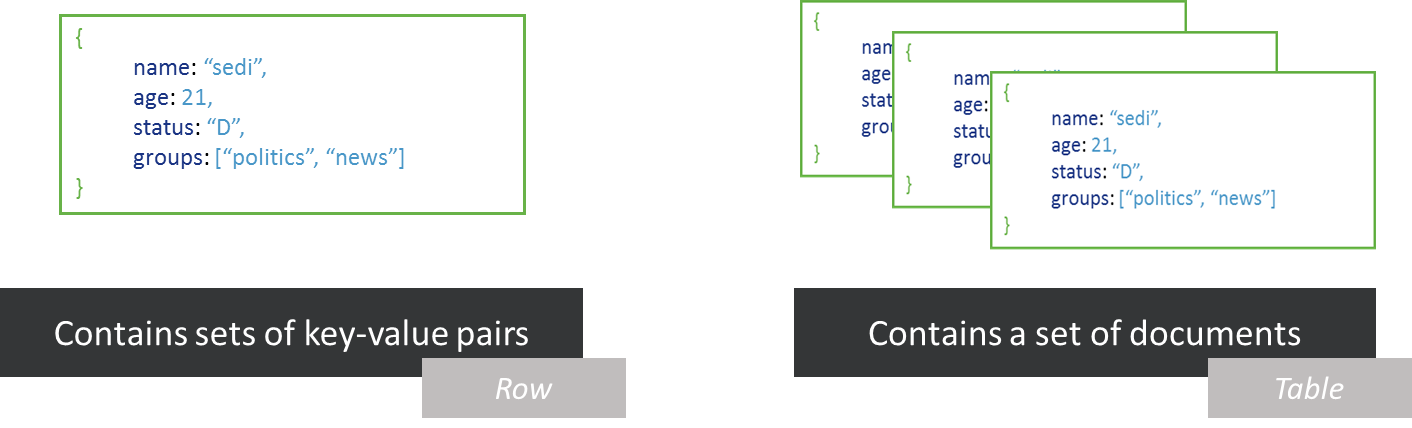
\includegraphics[width=\linewidth,keepaspectratio]{images/documentscollections.png}
\caption{Documents and collections}
\end{figure}

MongoDB stores data as Binary JSON documents also known as BSON. The documents can have different schemas, which means that the schema can change dynamically as the application evolves. Automatic sharding enables data in a collection to be distributed across multiple systems for horizontal scalability as data volumes increase\cite{Edward2015}. Additional, MongoDB doesn’t only support Key-Value operations. It allows complex queries, aggregations and secondary indexes that unlock the value in structured, semi-structured and unstructured data. One of MongoDB’s major features is the support for many types of queries like text search, range queries, geospatial queries over to MapReduce queries\cite{MongoDBInc.2013a}.
\\
MongoDB was created by Dwight Merriman and Eliot Horowitz, who had encountered development and scalability issues with traditional relational database approaches while building Web applications at DoubleClick, an Internet advertising company that is now owned by Google Inc. The database was released to open source in 2009 and is available under the terms of the Free Software Foundation's GNU AGPL Version 3.0 commercial license. However, the database is one of the most popular NoSQL databases and is used by several company like Bosch, Facebook, Expedia and so on\cite{Hows2013}.

\section{Use Cases: What is MongoDB for?}
This section will give you an insight between the features and potential of MongoDB and some problems that is suited to solve.
\\
Beginning with online and mobile Apps. Nowadays Companies want their business on their smartphones or access it from everywhere through the web. In comparison to RDMBS MongoDB addresses the upcoming challenges of these plans. Furthermore, MongoDB promises to make it easier than other alternatives. Requirements for going mobile or online are hard to manage. For example, different types of device like smartphone or wearables are creating new types of unstructured and semi-structured data. Another reason is the number of devices and users. Meanwhile, Response times must keep and provide the same User experience. So, Scalability has now a high priority. MongoDB tries to decrease the degree of difficulty for these Requirements. That is why MongoDB offers a flexible data model and rich query functionality. Therefore, MongoDB can manage any kind of data, no matter how dynamically the data changes. In addition to that, MongoDB’s development concentrates on scalability and can handle a lot of Users and data sets\cite{MongoDBInc.2013a}.
\\
Another Example for a suited use case is a catalog. Mention that almost anybody knows some requirements a Catalog must meet. Deleting, creating and changing items or their features or their attributes – only to mention few - are a standard set of Requirement of a catalog. Behind the scenes, we see a lot of challenges for a RDMS. There will be a lot of changes in the data, like new data and new metadata to your catalogs. We already talked about the untrusted and semi-structured in the first Use case. Again, we got the same problems with a RDBMS. How does MongoDB make it easier for developers? First, it is how the data is structured in MongoDB. With MongoDB’s JSON document model makes it easy to store different assets with different attributes in a single place. It also makes it simple to represent complex, hierarchical relationships. Schemas in MongoDB are self-describing. You can add new products and features and evolve the schema instantly, without taking the database down or impacting performance. Lastly an expressive query language, indexing, including text search and geospatial, and analytics provide flexible access to the data, no matter how the application, business or developer needs to find it\cite{MongoDBInc.2013a}.
\\
All in all, these are only few examples for use cases and for what MongoDB is. In general MongoDB claims to be suited for high flexible data schemas to provide the ability for data changes, structed, unstructured and semi structured data. Additionally, MongoDB eco system let developer spend less time for the design of models, entities, relationships and tables, and more time on the application\cite{MongoDBInc.2013a}.
\section{Datamodel}
Before designing a database, it is crucial to analyse the data and the requirements of the application. In contrast to relational databases there is no strongly recommended way to structure your data, like for example a normalized data model to avoid inconsistencies on updates. However, there are well established patterns which help developers to create their data model \cite{mdbinaction}. Later in this chapter, there will bw some examples for common design patterns. But at first, the following paragraphs will concentrate on the data concepts of MongoDB in detail.

\subsection{Databases and Collections}
As mentioned in the introduction, MongoDB is structured in databases, collections and documents. MongoDB provides a mongo shell to communicate with the database. The code snippets provided in this chaptered can be performed on the mongo shell \cite{mdbdocu}.

A Database can hold collections of documents. The creation of a database occurs automatically when the first document is pushed to a collection of this database. Thus, there is no command to create an empty database \cite{mdbdocu}. The following commands show how simply it is to select and create a new database by inserting its first document.

\begin{lstlisting}[frame=single, caption=Create Database, label=createdb]
use newDatabase
db.newCollection.insertOne( { value: 2 } )
\end{lstlisting}


This example also shows the process of creating a new collection. As the database, the collection is created as soon as the first document got inserted. Certainly, there is also a function to explicitly create a new collection with an option to pass parameters affecting the collections behaviour. In the example in Listing \ref{createcol}, a collection with limited number of documents is created. All options can be found in the MongoDB documentation \cite{mdbdocu}.

\begin{lstlisting}[frame=single, caption=Create Collection, label=createcol]
db.createCollection( 'newCollection', { max: 1000 } )
\end{lstlisting}

\subsection{Documents}
MongoDB stores documents in the BSON format. This format supports multiple datatypes. Many of them are common in the information technology, such as Double, String or Boolean. A full list would go beyond the scope of this book, but can be found in the BSON specification. In general, there are all types needed for object oriented programming \cite{bsonspec}. The chapter Queries and CRUD operations will treat the way BSON types can be used to query through documents. But before that, the concept of documents will be explained.

\subsection{Embedded Documents and Referencing}
The below example in Listing \ref{embdoc} shows how a document is structured. The field name \_id is reserved to be used as primary key. It has some special characteristics like being unique in the collection and immutable. To make sure this field is unique, it is recommended to use a unique ObjectId. If there is no value submitted with the document, an ObjectId is generated automatically \cite{mdbdocu}. 

\begin{lstlisting}[frame=single, caption=Embedded Documents, label=embdoc]
var newDocument = {
	_id: <ObjectId>,
	dateOfBirth: new Date('Jan 01, 1990'), 
	name: { 
        last:	 'Doe', 
        first: 'John' 
    },
	contact: {
		phone: '12345678',
		email: 'john@doe.com'
	}
}
\end{lstlisting}

Other fields can be added as needed. For example, a field containing the date of birth of a person. Or an object containing the first and last name and another object with contact details. This concept of containing objects inside a document is called embedded sub-documents and has its own strength and weaknesses \cite{mdbdocu}. It may be resulting in a performance growth if the application always needs the document with its whole embedded data. But one common pattern for MongoDB says to consider whether embedded data or referencing is more suitable for the given situation \cite{mdbinaction}. By referencing, the embedded data is stored in a separate document with a reference to its related document. This concept is the foundation for creating normalised data models. How this can be implemented for the document with John Doe can be seen in the code snippet in Listing \ref{refdoc}.

\begin{lstlisting}[frame=single, caption=Referencing Documents, label=refdoc]
var newPerson = {
	_id: <ObjectId1>,
	dateOfBirth: new Date('Jan 01, 1990'), 
}

var newName = {
	_id: <ObjectId2>,
	user_id: <ObjectId1>,	
    last:	'Doe', 
    first: 'John'
}

var newContact = {
    _id: <ObjectId3>,
    user_id: <ObjectId1>,	
    phone: '12345678',
	email: 'john@doe.com'

}
\end{lstlisting}

When deciding whether referencing is reasonable, the atomicity of write operations also influences this decision. In MongoDB atomicity is only guaranteed on document level. As no single write operation can affect more documents, a normalised data model cannot be updated with one atomic operation. At this point denormalised data models have benefits over normalised ones. However, another design pattern for MongoDB is to overthink your overall database selection if you need atomic, consistent, isolated and durable operations, also known as ACID principles \cite{mdbinaction}. 

\subsection{Validation}
MongoDB comes with a way to validate documents by itself. There are different ways to handle documents which do not match its validation criteria. By default, invalid documents are rejected with an error. A collection, which would check if the new document contains a date of birth, would look like the following in Listing \ref{valcol}. Furthermore, it is also possible the check the fields for a certain data type \cite{mdbdocu}.

\begin{lstlisting}[frame=single, caption=Validation for Collections, label=valcol]
db.createCollection( 'users', {
	validator: { 
	    $or: [ { 
	        dateOfBirth: { $exists: true } 
	    } 
        ] 
    }
}
\end{lstlisting}
		
\section{Queries and CRUD operations}
MongoDB has several queries and operations to manage its data. This chapter gives a short overview of the most important operations.

\subsection{Create (Insert)}
Before searching for or working with data, the database needs information that can be worked with. How documents can be created was introduced while treating how to create a new database. This command inserts one document into a collection and can be found again in the Listing \ref{insdoc}. But there are also commands to insert an array of documents at once \cite{mdbbasics}.

\begin{lstlisting}[frame=single, caption=Create (Insert), label=insdoc]
db.newCollection.insertOne( {name: 'John', age: 30} )
db.newCollection.insertMany( [ 
    {name: 'Max', age: 20},
    {name: 'Marie', age: 25} 
] )
\end{lstlisting}

\subsection{Read (Find)}
To find data stored in a MongoDB, operations to either find one or multiple documents can be used. This example in Listing \ref{findoc} shows both operations. The difference is that the second operations stops after the first result and it is generally advised if only one result is excepted. Of course, the results can also be filtered by field values as shown in line three, or sorted by values as shown in line four \cite{mdbbasics}.

\begin{lstlisting}[frame=single, caption=Read (Find), label=findoc]
db.newCollection.find()
db.newCollection.findOne()
db.newCollection.find( { 'name.last': 'Doe' } )
db.newCollection.find().sort( { 'name.first': 1 } )
\end{lstlisting}

\subsection{Update}
MongoDB also provides a function to update documents with three input parameters: the search criteria, the new object and options. It is important to understand that any fields that are not part of the new object are also removed from the old object, as it were completely rewritten. The option upsert implies to add any fields that do not exist yet. It is also possible to update multiple options that match the search criteria with one command \cite{mdbinaction}. An example for a basic update operation can be found in Listing \ref{upddoc}.

\begin{lstlisting}[frame=single, caption=Update, label=upddoc]
db.newCollection.update(
    { name: 'John' }, 
    { age: 21, name: 'John', lastname: 'Doe'  }, 
    { upsert: true } )
\end{lstlisting}

\subsection{Delete}

The last operation of CRUD examines the deletion of documents, collections or whole databases. The remove operation, as shown in line one of the code snippet in Listing \ref{deldoc}, removes all documents which match the criteria. The \_id field can help to be sure to only delete the right document. It can lead to conflicts if a documents is deleted without considering its references, because references from other documents will not change automatically \cite{mdbbasics}. Line 2 shows how to delete a collection and line 3 shows how to delete an entire database.

\begin{lstlisting}[frame=single, caption=Delete, label=deldoc]
db.newCollection.remove( { age: 20 } )
db.newCollection.drop()
db.dropDatabase()
\end{lstlisting}

\newcommand{\anfu}[1]{\glqq #1\grqq}
\newcommand{\anfuc}[3]{\anfu{#1}\cite[{#2}]{#3}}

\section{Architecture}
\subsection{Core Processes}\label{mdb-core}
The MongoDB server package comes up with three main processes:
\begin{itemize}
  \item mongod
  \item mongo
  \item mongos
\end{itemize}
\textit{Mongod} is the core database server. Once started, the \textit{mongod} listens by default on port 27017 for requests. It also manages the data format and performs all background operations. For administration the \textit{mondod} provides an HTTP interface, witch can be reached at the localhost on port 28017 (1000 higher than the default port). The data directory \textit{mongod} connects to is by default C:\textbackslash data\textbackslash db (or /data/db). This directory definitely has to exist and the default ports have to be free, otherwise the process fails to start \cite{Edward2015}.\\
The \textit{mongo} process is an interactive MongoDB shell. It gives the user the possibility to communicate with a running \textit{mongod} process via a JavaScript like query language. If running on the same host, it automatically connects to the \textit{mongod} process and a preinstalled test database \cite{Edward2015}.\\
The \textit{mongos} process is working like a routing service and is the basis for MongoDBs sharding ability that will be described later (\ref{mdb-sharding}). It holds the information about where the requested data is located and forwards the request from an application server to the right destination \cite{Edward2015}. \\
By running a \textit{mongod} process you already have a standalone deployment of MonogDB that can be accessed by a client. But in case of failure there is no redundancy or recovery, that prevents data loss, so its not recommended to use this in a production environment. To avoid this, replication is used to guard against hardware failure or database corruption. It also gives the possibility to perform normally high-impact maintenance with little or no impact \cite{Hows2013}.

\subsection{Replication}
\anfuc{MongoDB supports the replication of a database’s contents to another server in real time or near real time}{p. 285}{Hows2013}. For that MongoDB provides two different replication methods. The traditional \textit{Master/Slave Replication} and \textit{Replication Sets}.

\subsubsection{Master/Slave Replication}
In a Master/Slave setup one \textit{mongod} instance acts as a master, the others declared as slaves. All write and read operations are requested to the master and the slaves replicate the data of the master, but can't be requested by a client. If a failure occurs that forces the master to go down, the hole system can't be reached anymore. The data, till the last replication to the slaves, is saved, but can't be accessed until the master comes up again. \\
In MongoDB the master holds a capped collection called \textit{oplog}. The \textit{oplog} is an ordered history of all logical writes, that are executed within a defined time period. The operations stored in the \textit{oplog} in an idempotent way, so they can be performed multiple times without changing the result \cite{Edward2015}. That's useful when a slave runs into failure while executing the operations onto its data. In that case the replication process can be simply restarted. If the slaves syncing process last to long or the slave was down for a longer time, the oplog data could be deleted before the slave was able to synchronize \cite{Edward2015}. In that case the slave has to start a resync process. To avoid such a situation, the oplog length should be chosen in consideration of the slaves performance.\\
The configuration of MongoDB with a \textit{Master/Slave Replication} is only recommended for more than 50 nodes \cite{Edward2015}. At that point the next described replication method, the \textit{Replica Set}, is reaching its limits, because the communication overhead becomes to big.

\subsubsection{Replica sets}
In contrast to the \textit{Master/Slave Replication}, in a \textit{Replica Set} no fixed master is defined. Instead the nodes are declared as primary or secondary. Each node in a \textit{Replica Set} can become primary, but there is only one primary at a time, the others are secondaries. All write operations going through the primary, but read operations can also be performed by secondaries \cite{Edward2015}. The replication process works just like it does in a \textit{Master/Salve Replaction}, but if a primary goes down a new primary is elected out of the secondaries.

\subsubsection{Communication}
All nodes in a \textit{Replica Set} communicate with each other. As life sign they are sending a heartbeat signal to each node and getting back status replies of each node. Those replies contain information about the node, such as is he primary or secondary and what type of node he is. Each node can be assigned a certain number of votes and a priority.\\
This results in a various types of nodes:
\begin{itemize}
  \item \textbf{normal secondaries:} hold a copy of the primaries data, accept read requests and are primary candidates
  \item \textbf{priority-0-members:} secondaries that will never become primary
  \item \textbf{hidden-members:} priority-0-members that can't serve read request, because they are hidden for the client
  \item \textbf{delayed-members:} have a delay in synchronization to prevent human failure
  \item \textbf{arbiters:} don't hold data, they just solve ties in a election process
  \item \textbf{non-voting-members:} normal secondaries, but they can't vote
\end{itemize}
If the primary recognizes that the heartbeat of a secondary has stopped, he has to check if he still can reach the majority of the set. If it can't he demotes itself to secondary and starts a election process. Also the election process is started if a secondary recognizes the primary is down. All voting nodes now collect the for the election required information form the primary candidates. The election of a primary depends on various parameters. Important is, that the elected node has the most recent data of all nodes. The candidate with the most votes is promoted to primary. When the old primary comes up again, he will be a new secondary \cite{Edward2015,Hows2013}.

\subsubsection{Write Concerns and Read Preferences}\label{read-write}
MongoDB provides two important configurations to regulate consistency and availability. With \textit{write concerns} it's possible to configure a minimum number of secondaries, that have to replicate the data, before the client gets the success response. Figure \ref{write-concerns} shows how a write process would run, by configuring a minimum of one secondaries.
\begin{figure}[H]
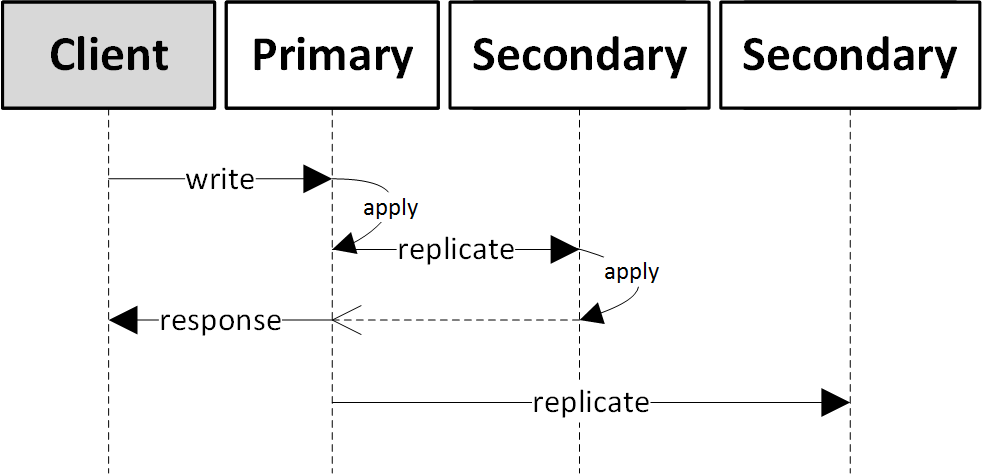
\includegraphics[width=\linewidth,keepaspectratio]{images/write-concern.png}
\caption{Write process with write concerns}
\label{write-concerns}
\end{figure}
\textit{Read preferences} allow the administrator to route read operations. They determine from which node a client is allowed to read. MongoDB supports five read preferences:
\begin{itemize}
  \item \textbf{primary:} all read operations are requested to the primary node
  \item \textbf{primaryPreferred:} read operations are requested to secondaries, if the primary is unavailable
  \item \textbf{secondary:} read operations are requested to secondaries
  \item \textbf{secondaryPreferred:} read operation are just requested to primary, if no secondary is available
  \item \textbf{nearest:} read operations are requested to the node with the lowest network latency
\end{itemize}
\cite{mdbdocu}
\subsection{Sharding}\label{mdb-sharding}
If the amount of data exceeds the capacity of a single database server, partitioning is needed to distribute the data on multiple servers. For MongoDB this ability is even more important, because it uses memory mapped file I/O to access its underlining data storage \cite{Hows2013}. MongoDB uses a horizontal partitioning mechanism called \textit{sharding}.\\
The data collection gets divided and distributed onto multiple servers called shards. Every shard is an independent database managed by multiple \textit{mongod} processes. All the shards are combined to one logical database. The partitioning and routing are managed by the earlier mentioned \textit{mongos} (\ref{mdb-core}) process. All write and read requests of an application are send to a \textit{mongos} process, that holds the information where the requested data is stored and forwards the requests to the responsible \textit{mongod} processes. The data is distributed based on a configured \textit{shard key} and chunk size. The metadata of a sharded cluster is stored on special config servers, where the \textit{mongos} processes can obtain the routing information \cite{Edward2015,Hows2013}.

\subsection{Summary}
Figure \ref{arch-example} describes one possible deployment architecture, that contains all in this section mentioned artifacts. Clients can connect to a \textit{mongos} process, running on an application server. This process forwards the requests, based on the information stored on the \textit{config servers}, to the right shard. A shard is an replica set, containing several \textit{mongod} processes. The \textit{shard key} in this example is the year. So Shard-1 contains all data from 1999 til 2009 and Shard-2 contains the data from 2009 til now. 
\begin{figure}[H]
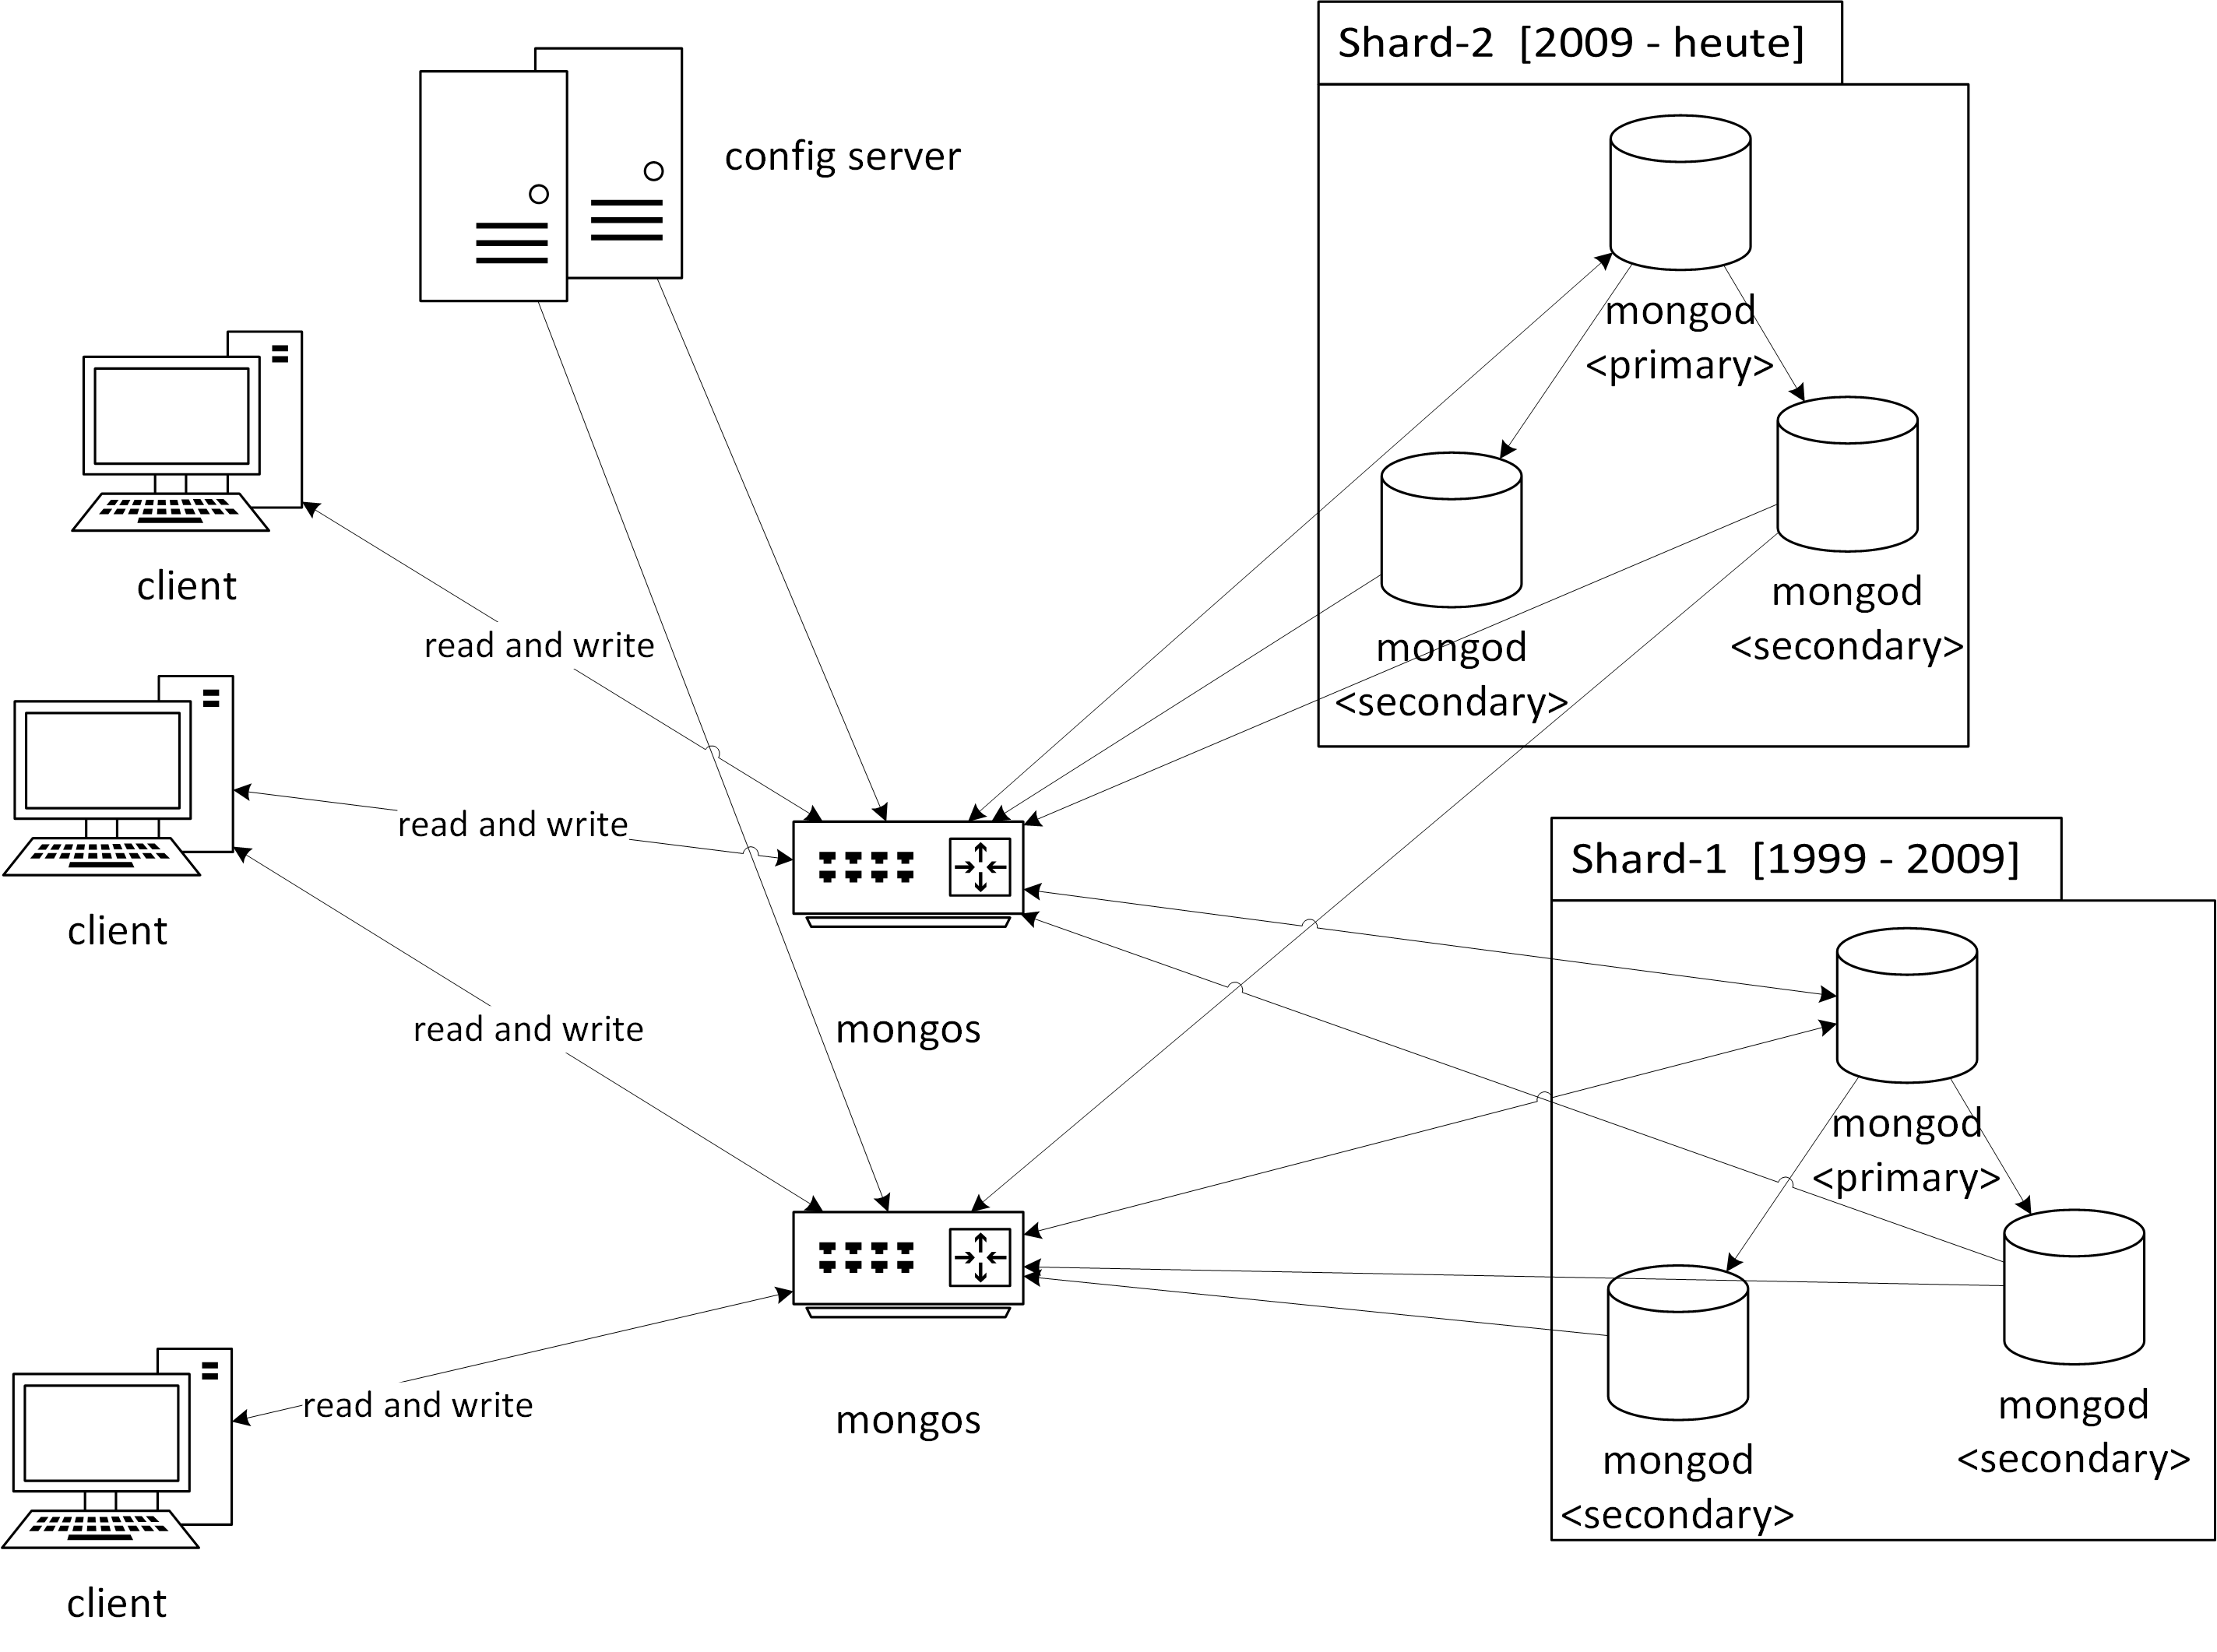
\includegraphics[width=\linewidth,keepaspectratio]{images/sharding.png}
\caption{MongoDB Architecture Example}
\label{arch-example}
\end{figure}

\section{Performance}
\subsection{Performance measurement introduction}
Before a performance measurement or comparison between database systems can be made, it is necessary to define the performance indicators. Depending on the use-case of the measured databases the results can be completely different. For example a real-time system is a lot more dependent on access times, latency and fast updates for concurrent users. A scientific database has to be fast at processing complex queries with joints and preprocessing routines like aggregation \cite{Neil_O}. Of course the benchmark should be implemented to test the performance of a database system in a way that reflects your usage in the future.
\\\\
For database systems there is a council called the TPC . This organization tests different database systems on physical and virtual machines and scores them by performance. The performance indicators can be seen on their website and there are different benchmarks depending on the use-case of the system \cite{_tpc.org.}. 
\\\\
Another standardized benchmark for database implementations is the Wisconsin Benchmark. This was one of the first standardized benchmarks and was made for relational databases. The test contains of inserts, selections, joints and projections. For further details on this benchmark, see the paper \cite{DeWitt_The_1991}.
\\\\
This paper will summarize MonogDB performance compared to other popular NoSQL and SQL  databases.

\subsection{Influencing factors to database performance}
All the results provided by this paper are dependent on the underlying hardware used. Depending on the host system for the database application, the performance can vary a lot \cite{Lee_W._2009}. Examples for big performance factors are available memory, processor speed and the used storage.
\\\\
For evaluation which database system should be used, it is important to know on what kind of hardware the production system will run. This is due to the fact, that different database systems were developed to meet certain performance goals on different hardware. Therefore some databases scale well with more memory and memory bandwidth since they try to cache a lot of the data in system memory. But there are also databases which try to be very lightweight on memory for low end systems or massive I/O  operations \cite{Boncz_Database_1999}.
\\\\
Nearly all databases are reliant on the used storage. This storage is the only way to keep the data, even when the system is turned off. Even In-memory databases use the persistent storage to save their current data \cite{Wang_Main_2001}. As transactions ultimately have to be written to the storage, this becomes the biggest bottleneck. With traditional HDDs having a high latency when accessing random data, which happens frequently on a database system, the introduction of SSDs  eliminated those problems. Benchmarks done on traditional HDD storage can be translated most of the time to SSDs since all databases will perform better but should stay at the same relative performance.
\subsection{NOSQL compared to SQL databases}
It is often one of the first question, when talking about database performance. SQL or NOSQL, which one is faster? Comparing those two types of databases generally, is not really useful. The way how data is stored is completely different and the use-case defines if SQL or NOSQL fits better.
\\\\
A good example for the difference of these two types is Twitter. They use a NOSQL database for all the tweets. Although Twitter is using MySQL heavily. The reason for this is easy to explain. A tweet contains some sort of content like text or images and a lot of additional information like hashtags, user and topics. Storing that data in a relational, normalized way, it would take a lot of tables and joins to represent a tweet . All hashtags would be referenced over multiple tables. These joins take time and since Twitter is a real time platform, latency should be low \cite{Weil_21}.
\\\\
In contrast the NOSQL implementation is way easier. The complete Tweet is stored as a document. The hashtags and links are stored in the same document in a key value manner. Now when you want to read 100 Tweets, in a NOSQL context, this can be done by one simple query. In a relational model, complex joins for each Tweet would be necessary. In such a scenario performance is obviously on the NOSQL side, but only because the use-case is well suited for non-relational models.
\subsection{MongoDB performance}
This paper will be limited to benchmarks of low level functions for databases. These functions are: reads, writes and deletions. Performance is measured between MongoDB and MariaDB. MariaDB is a SQL database and as previously mentioned, general comparisons between NOSQL and SQL are not useful. In this case two implementations of SQL and NOSQL are compared which is relevant when the use-case can be implemented by both designs without drawbacks. In such a scenario, raw performance is a valid factor.
In addition to the benchmark implemented by the author of this section, another one is used for validity and a broader overview. The referenced paper contains additional databases.
\\\\
The following performance test were performed, using NodeJS. For MongoDB connectivity the official MongoDB driver  was used. The same applies for the MariaDB driver . The driver selection can cause huge performance differences. There are several MariaDB drivers for NodeJS and of course other programming languages. Therefore comparisons of database performance should be done, using the same programming language \cite{_mscdex.}. The inserted data contains just an id represented by an integer.
\begin{figure}[H]
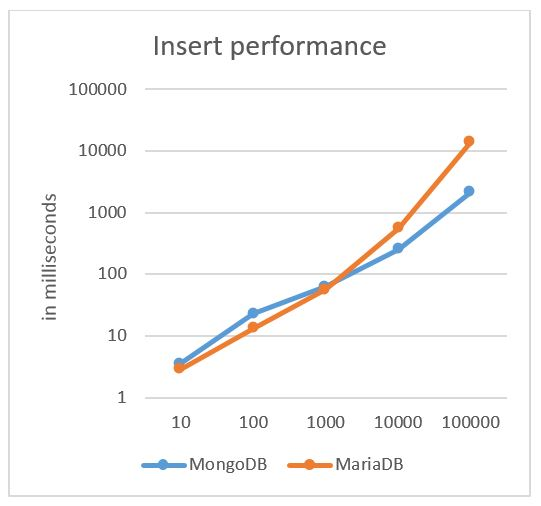
\includegraphics[width=\linewidth,keepaspectratio]{images/Performance_Inserts.JPG}
\caption{Insert MongoDB vs MariaDB}
\end{figure}
\begin{figure}[H]
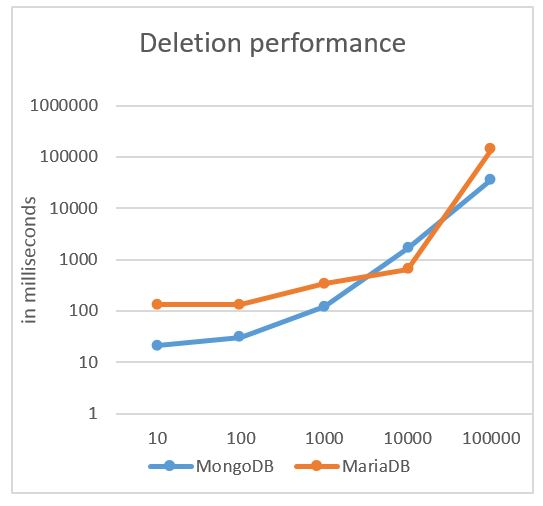
\includegraphics[width=\linewidth,keepaspectratio]{images/Performance_Deletion.JPG}
\caption{Deletion performance}
\label{arch-example4}
\end{figure}

The numbers show an interesting result. In the insert test MongoDB performs worse than MariaDB just slightly up to the point of 1000 inserts. After that point MariaDB falls behind. With increasing number of inserts the performance leap of MongoDB increases a lot. A reason for this could be some kind of overhead for inserts on MongoDB, further investigation is needed to evaluate the results and the cause. A similar behavior can be seen on deletion test.
\\\\
The following performance results are provided by the paper \cite{Li_A_2013}
\begin{figure}[H]
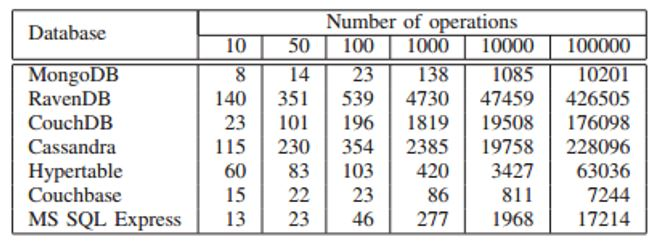
\includegraphics[width=\linewidth,keepaspectratio]{images/Performance_Reads.JPG}
\caption{Time for read operations in milliseconds}
\label{arch-example2}
\end{figure}
\begin{figure}[H]
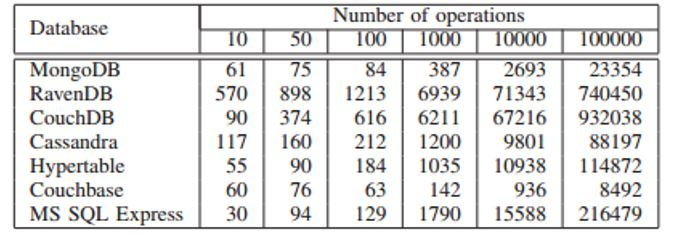
\includegraphics[width=\linewidth,keepaspectratio]{images/Performance_Writes.JPG}
\caption{Time for write operation in milliseconds}
\label{arch-example3}
\end{figure}
\begin{figure}[H]
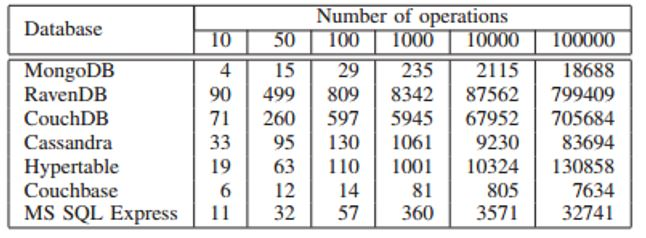
\includegraphics[width=\linewidth,keepaspectratio]{images/Performance_Delete.JPG}
\caption{Time for delete operation in milliseconds}
\label{arch-exampl1}
\end{figure}

Interestingly the benchmarks from the paper show similar results on write performance when comparing the SQL implementation and MongoDB. After 100 writes MongoDB performs better. When comparing to other NoSQL databases, MongoDB is always in the upper half of the field. So it can be said, that this database should be suited well for demanding applications and performance shouldn't be a major problem. 
\\\\
These statements only apply for single instance usage. Since MongoDB uses a single master architecture for multiple instances, throughput will be less than database systems that trade consistency for performance. Using sharded servers can increase performance for horizontal scaling. With this addition, MonngoDB is also very usable for scientific applications with high amounts of I/O and data \cite{Dede_Performance_2013}.




\section{MongoDB and Big Data}
In terms of Mobile Applications, IoT, Industry 4.0 and cloud-computing, data is vast, unstructured, sometimes unwieldy and complicated. In this context, Big Data is identified by its velocity, variety and volume. Therefore, requirement and expectations has changed how to store, process and analyze data. It has led to the development of NoSQL databases such as MongoDB\cite{MongoDBInc.2013}.
\\
However, in the era of Big Data, there a 2 kind of database solutions for facing Big Data. We distinguish operational Big Data Systems and analytical Big Data solutions. Features of Operational Big Data Systems provides real-time, interactive, dynamic workloads that ingest and store data. MongoDB belongs to this category and is a popular technology for operational Big Data applications\cite{MongoDBInc.2013}.
\\
On the other hand, Analytical Big Data technologies are useful for retrospective, sophisticated analytics of your data. A most-known example of an Analytical Big Data technology is Apache Hadoop. Hadoop is designed for storing and processing large sets of data on a distributed environment based on commodity servers and storage. It is an open-source Apache project, which consists of a distributed file system called HDFS (Hadoop Distributed File System) and a data processing and execution model called MapReduce\cite{Wadkar2014}.
\\
Choosing between operational and analytical Big Data solution isn’t the right way of thinking about facing this Decision. Many organizations are harnessing the power of Hadoop and MongoDB together to create complete big data applications. At the one hand, MongoDB powers the online, real time operational application, serving business processes and end-users, exposing analytics models created by Hadoop to operational processes. At the other hand, Hadoop consumes data from MongoDB, blending it with data from other sources to generate sophisticated analytics and machine learning models. Results are loaded back to MongoDB to serve smarter and contextually-aware operational processes – i.e., delivering more relevant offers, faster identification of fraud, better prediction of failure rates from manufacturing processes\cite{MongoDBInc.2013}.
\\
In the following, you see a Figure which shows a Design pattern how to combine these two technologies to be ready for a Big Data environment:
\begin{figure}[H]
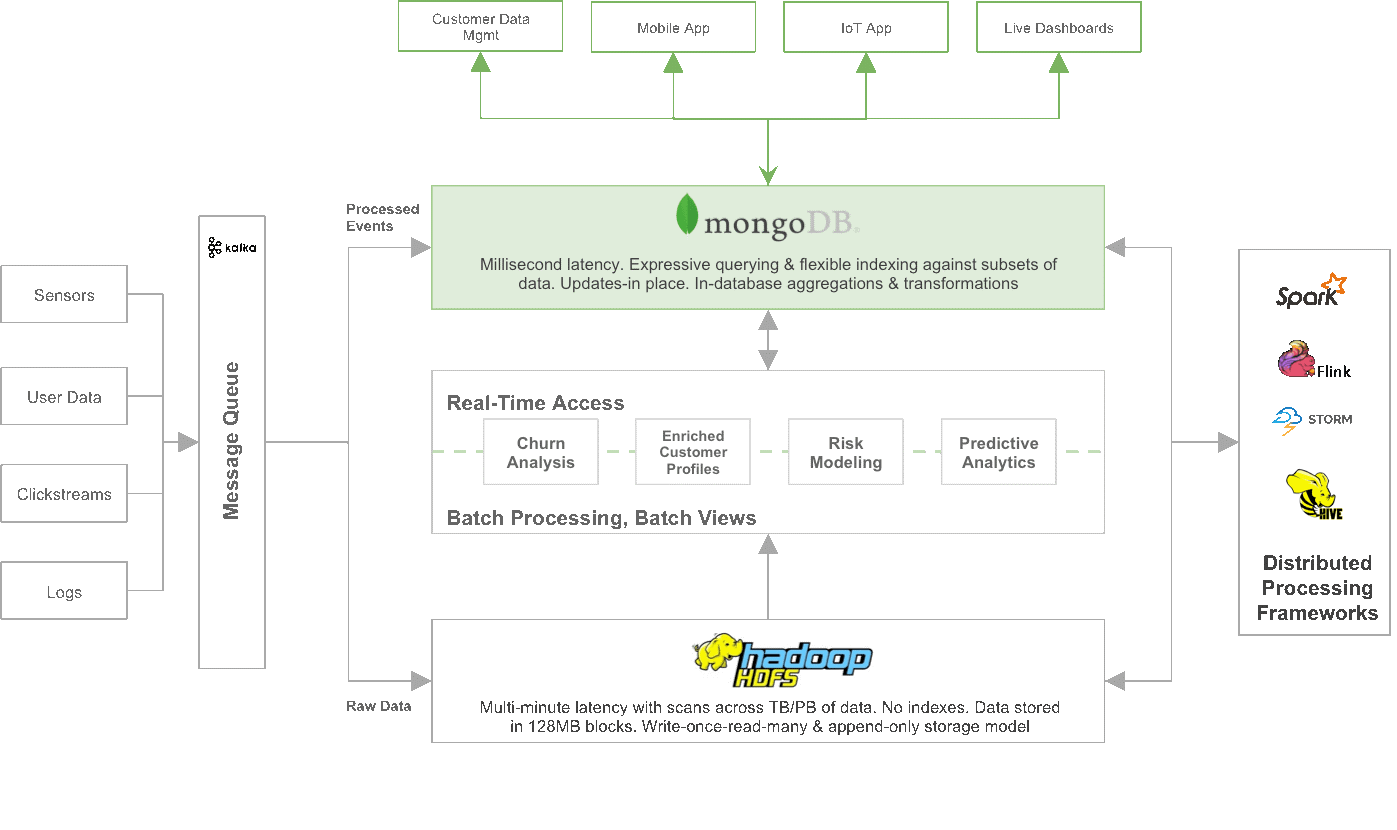
\includegraphics[width=\linewidth,keepaspectratio]{images/bigdata.png}
\caption{Design pattern for integrating MongoDB with Data Lake~\protect\cite{MongoDB2016}}
\end{figure}

\section{Conclusion}
All in all, MongoDB is a powerful and popular documented-oriented database. It comes with a lot of features, which meets the modern-day requirements and challenges for business applications, platforms and the web. 
The examples about the MongoDB data model, queries and CRUD operations showed how easy it is for developers to setup and work with this database. MongoDB is also very flexible in terms of extending the structure of documents. However, it is strongly recommended to consider the usage of common patterns to create a strong and future-proof data model. The usage of patterns will also help developers to understand a given database structure and work together on larger projects.
Even in a big data context MongoDB is a good choice for big data applications. That is why you will find a lot of companies and startups using MongoDB in their development.

\subsection{MongoDB in CAP-Theorem}
In a single server or Master/Slave configuration MongoDB prioritize consistency over availability. That might be the reason why in most literature MongoDB is positioned at CP-side of the CAP-Theorem. But in \textit{Replica Sets} it is possible to trade some of the consistency for a higher availability, by configuring \textit{read preferences} (\ref{read-write}). By allow reading from secondaries, there is no way to ensure the client is reading consistent data. \anfuc{This behavior is characterized as eventual consistency, witch means that although the secondary's state is not consistent with the primary node state, it will become consistent over time}{p. 108}{Edward2015}. With \textit{write concerns} (\ref{read-write}) it is possible to obviate inconsistent reads happen to often, by ensure that a minimum number of secondaries is consistent. \\
Figure \ref{mongodb-cap} describes how the three values change depending on the configuration. The partition tolerance is always fulfilled, because MongoDBs architecture is designed that way. By allow reading from secondaries availability will be increased at the expense of consistency and some consistency can be recovered using \textit{write concerns}. But availability is always limited to reading, so it can never be fulfilled for all aspects of an application.
\begin{figure}[H]
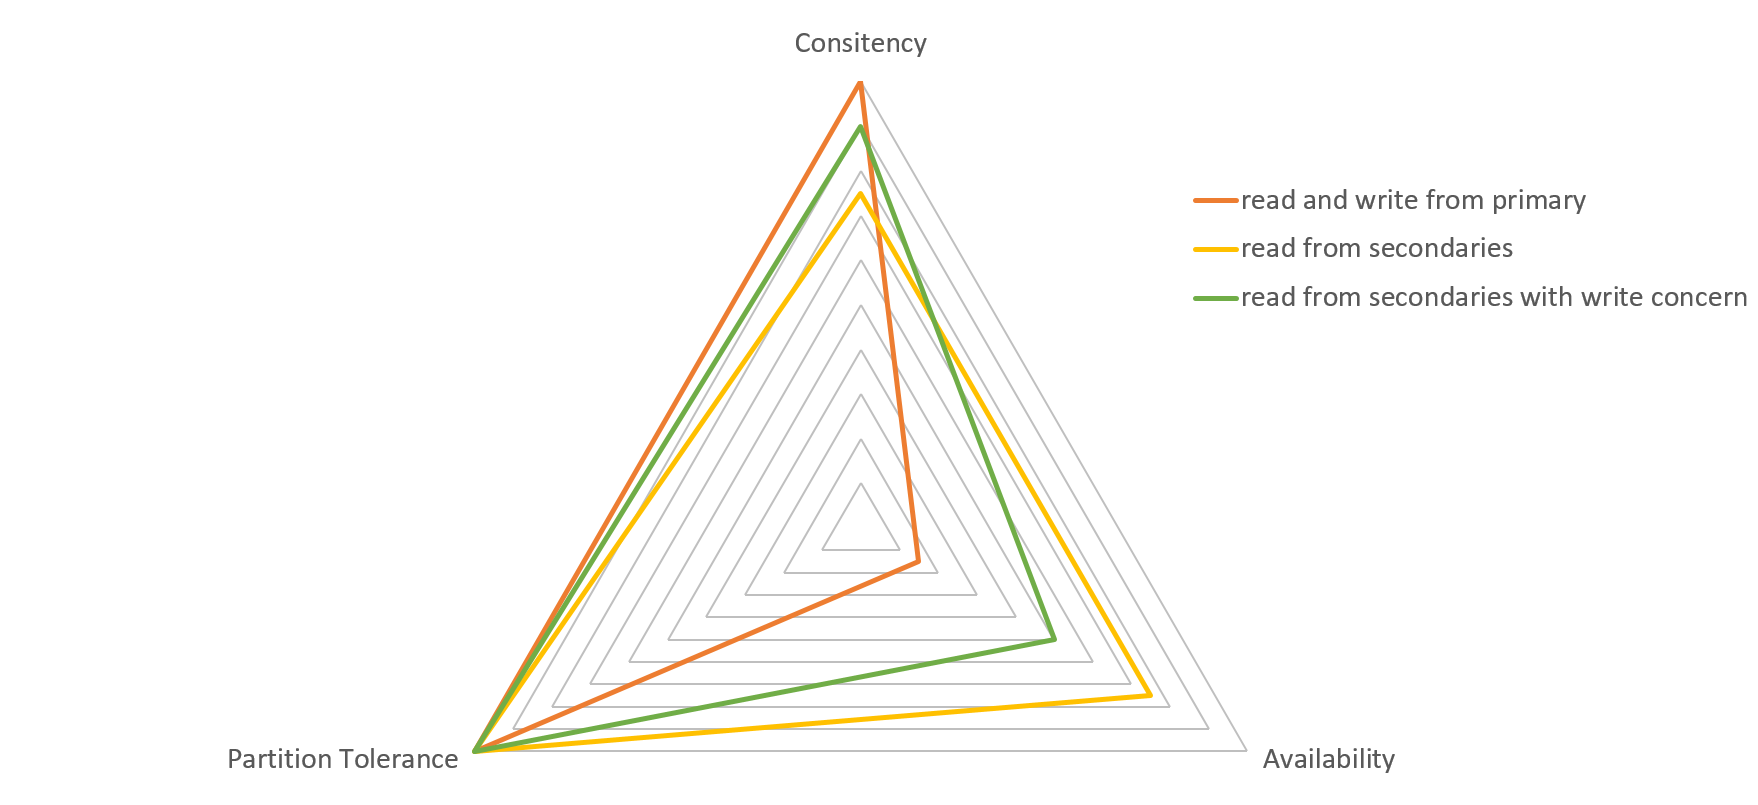
\includegraphics[width=\linewidth,keepaspectratio]{images/mongodb-cap.png}
\caption{Write process with write concerns}
\label{mongodb-cap}
\end{figure}

	
	\clearpage
		
	\pagenumbering{roman}
	
	% Literaturverzeichnis
	\cleardoublepage
  \bibliographystyle{apacite}
  \bibliography{bibliographie}
	\newpage\null\thispagestyle{plain}\newpage
	
	% Glossar
	\printglossary[style=altlist,title=\langglossar]
	%%!TEX root = ../dokumentation.tex

%
% vorher in Konsole folgendes aufrufen:
%	makeglossaries makeglossaries dokumentation.acn && makeglossaries dokumentation.glo
%

%
% Glossareintraege --> referenz, name, beschreibung
% Aufruf mit \gls{...}
%
\newglossaryentry{Glossareintrag}{name={Glossareintrag},plural={Glossareinträge},description={Ein Glossar beschreibt verschiedenste Dinge in kurzen Worten}}

\newglossaryentry{Commodity-Hardware}{name={Commodity-Hardware},description={\flqq Computer hardware that is affordable and easy to obtain. Typically it is a low-performance system that is IBM PC-compatible and is capable of running Microsoft Windows, Linux, or MS-DOS without requiring any special devices or equipment.\frqq\footcite{Beal.2015}}}

\newglossaryentry{Git}{name={Git},plural={Git},description={Git ist ein kostenloses System zur Versionskontrolle für kleine wie auch sehr große Projekte. ({\url{http://git-scm.com/}})}}

\newglossaryentry{NetBeans}{name={NetBeans},plural={NetBeans},description={The Smarter and Faster Way to Code Quickly and easily develop desktop, mobile and web applications with Java, HTML5, PHP, C/C++ and more. NetBeans IDE is FREE, open source, and has a worldwide community of users and developers. ({\url{https://netbeans.org}})}}

\newglossaryentry{Maven}{name={Maven},plural={Maven},description={Apache Maven is a software project management and comprehension tool. Based on the concept of a project object model (POM), Maven can manage a project’s build, reporting and documentation from a central piece of information. \\ ({\url{http://maven.apache.org/}})}}

\newglossaryentry{Nagios}{name={Nagios},plural={Nagios},description={Nagios Is The Industry Standard In IT Infrastructure Monitoring. Achieve instant awareness of IT infrastructure problems, so downtime doesn't adversely affect your business. Nagios offers complete monitoring and alerting for servers, switches, applications, and services. \\ ({\url{https://www.nagios.org}})}}

\newglossaryentry{Zabbix}{name={Zabbix},plural={Zabbix},description={Zabbix is the ultimate enterprise-level software designed for real-time monitoring of millions of metrics collected from tens of thousands of servers, virtual machines and network devices. Zabbix is Open Source and comes at no cost. \\ ({\url{http://www.zabbix.com}})}}

\newglossaryentry{Bootstrapping}{name={Bootstrapping},description={\flqq The computer term bootstrap began as a metaphor in the 1950s. In computers, pressing a bootstrap button caused a hardwired program to read a bootstrap program from an input unit. The computer would then execute the bootstrap program, which caused it to read more program instructions. It became a self-sustaining process that proceeded without external help from manually entered instructions. As a computing term, bootstrap has been used since at least 1953.\frqq\footcite[S. 1273]{Buchholz.1953}}}

\newglossaryentry{Generic}{name={Generic},plural={Generics},description={Ein Interface oder eine Klasse kann mit einem oder mehreren Parametern, den sog. Generics, definiert werden, welche zusätzliche Typangaben enthalten. Diese werden in spitzen Klammern notiert. Generics führen implizit einen Typumwandlung durch, welcher ohne Generics explizit erfolgen müsste\footcite[Vgl.][S. 4 f.]{Naftalin.2006}}}

\newglossaryentry{Plugin}{name={Plugin},plural={Plugins},description={\flqq Zusatzprogramm, welches über eine vordefinierte Schnittstelle in ein Basisprogramm eingebunden wird und dessen Funktionsumfang erweitert. [...] [Stammen] oftmals von anderen Herstellern als das Basisprogramm. [...] Plug-ins sind oft aus eigenständigen Programmen entstanden und können deshalb [...] i.d.R. auch ohne das Basisprogramm verwendet werden\frqq\footcite[]{Lackes.2015}}}
	

\end{document}
